% Created 2024-09-28 Sat 00:27
% Intended LaTeX compiler: pdflatex
\documentclass[11pt]{article}
\usepackage[utf8]{inputenc}
\usepackage[T1]{fontenc}
\usepackage{graphicx}
\usepackage{longtable}
\usepackage{wrapfig}
\usepackage{rotating}
\usepackage[normalem]{ulem}
\usepackage{amsmath}
\usepackage{amssymb}
\usepackage{capt-of}
\usepackage{hyperref}
\usepackage{siunitx}
\usepackage{array}
\setlength{\parindent}{0em}
\author{Hankertrix}
\date{\today}
\title{MA3010 Thermodynamics and Heat Transfer Cheat Sheet (Thermodynamics Section)}
\hypersetup{
 pdfauthor={Hankertrix},
 pdftitle={MA3010 Thermodynamics and Heat Transfer Cheat Sheet (Thermodynamics Section)},
 pdfkeywords={},
 pdfsubject={},
 pdfcreator={Emacs 29.4 (Org mode 9.6.15)}, 
 pdflang={English}}
\begin{document}

\maketitle
\setcounter{tocdepth}{2}
\tableofcontents \clearpage
\section{Definitions}
\label{sec:orgf0c7d8e}

\subsection{Thermodynamics}
\label{sec:orgdb883b3}
\begin{itemize}
\item Thermodynamics analyses the \textbf{amount} of energy (heat or work done) as a system undergoes a process from one equilibrium state to another.
\item It only considers the end states in equilibrium and DOES NOT provide information (like time taken) from initial to final state.
\end{itemize}

\subsection{Heat transfer}
\label{sec:org6e13ab1}
\begin{itemize}
\item Heat transfer analyses the \textbf{rate} of energy transfer and \textbf{temperature distribution} during a process.
\item It is related to time and non-equilibrium states when a temperature gradient exists.
\end{itemize}

\subsection{Change in specific internal energy of an ideal gas}
\label{sec:org89c2fc9}
\[\Delta u = c_{\text{v, avg}} (T_2 - T_1)\]

Where:
\begin{itemize}
\item \(\Delta u\) is the change in specific internal energy of an ideal gas
\item \(c_{\text{v, avg}}\) is the specific heat capacity of the ideal gas at constant volume
\item \(T_2\) is the final temperature
\item \(T_1\) is the initial temperature
\end{itemize}

\subsection{Change in specific enthalpy of an ideal gas}
\label{sec:orgf8d708a}
\[\Delta h = c_{\text{p, avg}} (T_2 - T_1)\]

Where:
\begin{itemize}
\item \(\Delta h\) is the change in specific enthalpy of an ideal gas
\item \(c_{\text{p, avg}}\) is the specific heat capacity of the ideal gas at constant pressure
\item \(T_2\) is the final temperature
\item \(T_1\) is the initial temperature
\end{itemize}

\subsection{Quality (dryness fraction) (\(x\))}
\label{sec:org9d43f2d}
Dryness fraction, or quality, \(x\), is the proportion of vapour and liquid by mass in a two-phase mixture. The quality is 0 at the saturated liquid volume (\(v_f\)) and 1 at the saturated gas volume (\(v_g\)). A two-phase system can be treated as a homogenous mixture for convenience.

\[x = \frac{m_{vapour}}{m_{total}} = \frac{m_g}{m_f + m_g}\]

Where:
\begin{itemize}
\item \(x\) is the quality or dryness fraction
\item \(m_{vapour}\) is the mass of vapour
\item \(m_{total}\) is the total mass
\item \(m_g\) is the mass of vapour
\item \(m_f\) is the mass of liquid
\end{itemize}

\subsubsection{Specific entropy in terms of quality (\(s\))}
\label{sec:org3e1aa72}
\[s = (1 - x)s_f - xs_g = s_f + xs_{fg}\]

Where:
\begin{itemize}
\item \(s\) is the specific entropy
\item \(s_f\) is the specific entropy of the saturated liquid
\item \(s_g\) is the specific entropy of the saturated vapour
\item \(s_{fg}\) is the specific entropy of the mixture at evaporation, where \(s_{fg} = s_g - s_f\)
\end{itemize}

 \newpage

\subsubsection{Quality in terms of specific entropy (\(x\))}
\label{sec:orgb144a7c}
\[x = \frac{s - s_f}{s_{fg}}\]

The same formula can also be used for other properties, like specific internal energy (\(u\)), specific enthalpy (\(h\)) or specific volume (\(u\)).

Where:
\begin{itemize}
\item \(x\) is the quality
\item \(s\) is the specific entropy of the mixture
\item \(s_f\) is the specific entropy of the saturated liquid
\item \(s_g\) is the specific entropy of the saturated vapour
\item \(s_{fg}\) is the specific entropy of the mixture at evaporation, where \(s_{fg} = s_g - s_f\)
\end{itemize}

\subsection{Second Law of Thermodynamics}
\label{sec:orgea7f7ba}

\subsubsection{Introduction}
\label{sec:org896380f}
\begin{enumerate}
\item It identifies the direction of processes.
\item It determines the theoretical limits for the performance of engineering systems, like heat engines and refrigerators.
\begin{itemize}
\item Defines "perfection" for thermodynamic processes
\item Used as a benchmark for real engineering systems
\end{itemize}
\item It asserts that energy has \textbf{quality} as well as quantity. It determines the degree of degradation of energy during a process.
\begin{itemize}
\item Energy at a high temperature has better quality than the same energy at a low temperature.
\end{itemize}
\item Predicts degree of completion for chemical reactions.
\begin{itemize}
\item A process is completed when entropy stops increasing.
\end{itemize}
\end{enumerate}

\subsection{Thermal energy reservoirs}
\label{sec:orgce20361}
\begin{itemize}
\item A thermal energy reservoir is a hypothetical body with a relatively large \textbf{thermal energy capacity (mass \(\boldsymbol{\times}\) specific heat)} that can absorb or supply finite amounts of heat \textbf{without undergoing any change in temperature}.
\item In practice, large bodies of water (oceans, lakes and rivers) and the atmospheric air can be modelled as thermal energy reservoirs.
\end{itemize}
\[Q = mc \Delta T\]

\subsubsection{Heat source}
\label{sec:orgc20327d}
A heat source supplies heat energy. Some examples include the Sun, a furnace, etc.

\subsubsection{Heat sink}
\label{sec:org9b294e6}
A heat sink absorbs heat energy. Some examples include the river, atmosphere, etc.

\subsection{Heat engines}
\label{sec:org75a5078}
\begin{itemize}
\item Work is easily converted into other forms of energy such as heat, but the reverse is more difficult.
\item Heat engines convert heat to work.
\begin{enumerate}
\item Receive heat from a high-temperature source.
\item Convert part of the heat received to work.
\item Reject the remaining waste heat to a low-temperature sink.
\item Operate on a \textbf{cycle}.
\end{enumerate}
\item One example is a steam power plant.
\begin{itemize}
\item \(Q_{in}\) is the heat supplied to the steam in the boiler.
\item \(W_{out}\) is the work extracted from the steam in the turbine.
\item \(Q_{out}\) is the heat rejected by the steam in the condenser.
\item \(W_{in}\) is the work required to pump water into the boiler.
\end{itemize}
\item Net output from the heat engine is:
\end{itemize}
\[W_{\text{net, out}} = W_{out} - W_{in}\]

\subsubsection{Diagram}
\label{sec:orgcbe229b}
\begin{center}
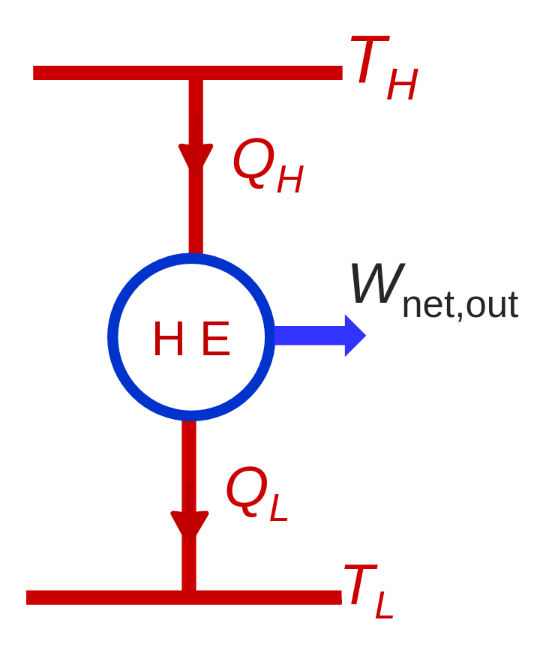
\includegraphics[width=.9\linewidth]{./images/heat-engine-diagram.png}
\end{center}

Where:
\begin{itemize}
\item \(T_H\) is the temperature of the high temperature reservoir
\item \(Q_H\) is the heat transferred from the high temperature reservoir
\item \(T_L\) is the temperature of the low temperature reservoir
\item \(Q_L\) is the heat transferred from the low temperature reservoir
\item \(W_{\text{net, out}}\) is the net work output of the heat engine
\end{itemize}

\subsubsection{Energy balance}
\label{sec:orgb0326c8}
From first law:
\[Q + W = \Delta U\]

For a cycle:
\[Q + W = 0\]
\[Q_H + (-Q_L) + (-W_{\text{net, out}}) = 0\]
\[W_{\text{net, out}} = Q_{in} - Q_{out}\]

Where:
\begin{itemize}
\item \(Q\) is the heat energy input into the system
\item \(W\) is the work done on the system
\item \(Q_H, Q_{in}\) is the heat energy input from the high temperature reservoir (H for high temperature)
\item \(Q_L, Q_{out}\) is the heat energy output from the low temperature reservoir (L for low temperature)
\item \(W_{\text{net, out}}\) is the net work output
\end{itemize}

\subsubsection{Thermal efficiency (\(\eta\))}
\label{sec:org8e5519a}
A measure of how well a heat engine converts heat input into useful work:
\[\text{Thermal Efficiency} = \frac{\text{Net work output}}{\text{Total heat input}}\]
\[\eta_{th} = \frac{W_{\text{net, out}}}{Q_{in}} = 1 - \frac{Q_{out}}{Q_{in}}\]
\[\eta_{th} = \frac{W_{\text{net, out}}}{Q_{H}} = 1 - \frac{Q_L}{Q_H}\]

 \newpage

\subsection{Kelvin-Planck statement}
\label{sec:org8e74979}
\[\eta_{th} = 1 - \frac{Q_L}{Q_H}\]
\begin{itemize}
\item If \(Q_L = 0\), the heat engine will have 100\% efficiency.
\item However, there is always waste heat produced.
\item The cycle cannot be completed without rejecting heat to a low-temperature sink.
\end{itemize}

Hence, it is impossible for any device that operates on a cycle to receive heat from a single reservoir and produce a net amount of work. Even theoretically perfect heat engines don't have an efficiency of 100\%.

This statement is equivalent to the Clausius statement.

 \newpage

\subsection{Reverse heat engine (refrigerators and heat pumps)}
\label{sec:org6e524c6}

\subsubsection{Diagram}
\label{sec:org581ad69}
\begin{center}
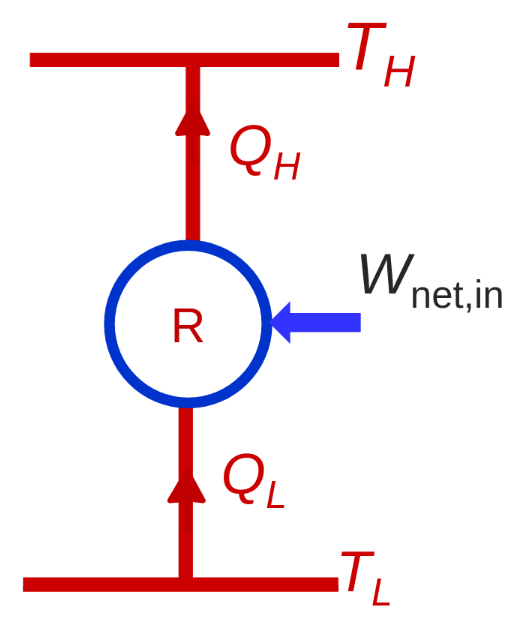
\includegraphics[scale=1.1]{./images/reverse-heat-engine-diagram.png}
\end{center}

Where:
\begin{itemize}
\item \(T_H\) is the temperature of the high temperature reservoir
\item \(Q_H\) is the heat transferred from the high temperature reservoir
\item \(T_L\) is the temperature of the low temperature reservoir
\item \(Q_L\) is the heat transferred from the low temperature reservoir
\item \(W_{\text{net, in}}\) is the net work input of the heat engine
\end{itemize}

\subsubsection{Refrigerators and heat pumps}
\label{sec:org4c75903}
\begin{itemize}
\item Heat transfer form high temperatures to low temperatures by nature
\item The opposite can only be achieved using refrigerators and heat pumps
\item Refrigerators and heat pumps are examples of "reverse heat engines"
\item They operate in a cycle
\item The working fluid is called a refrigerant
\item Vapour-compression refrigeration system is the most commonly used cycle
\item \(W_{in}\) is the work input to compressor to compress refrigerant from low to high pressure
\item \(Q_H\) is the heat rejected by the refrigerant in the condenser
\item \(Q_L\) is the heat absorbed by refrigerant in evaporator
\end{itemize}

\subsubsection{Energy balance}
\label{sec:orgbcefcf1}
\[W_{\text{net, in}} = Q_H - Q_L\]

\subsection{Coefficient of Performance (\(COP\))}
\label{sec:org497227b}
\begin{itemize}
\item The efficiency of refrigerators and heat pumps is expressed in terms of \textbf{coefficient of performance}.
\item The formula depends on the function of the machine:
\end{itemize}
\[\text{Coefficient of Performance} = \frac{\text{Desired output}}{\text{Required input}}\]

 \newpage

\subsubsection{Refrigerator}
\label{sec:org13ffe87}
Getting the coefficient of performance:
\[COP_R = \frac{Q_L}{W_{\text{net, in}}}\]

From the energy balance:
\[W_{\text{net, in}} = Q_H - Q_L\]

Hence:
\[COP_R = \frac{Q_L}{Q_H - Q_L} = \frac{1}{\frac{Q_H}{Q_L} - 1}\]

\subsubsection{Heat pump}
\label{sec:orgc218ec6}
Getting the coefficient of performance:
\[COP_{HP} = \frac{Q_H}{W_{\text{net, in}}}\]

From the energy balance:
\[W_{\text{net, in}} = Q_H - Q_L\]

Hence:
\[COP_{HP} = \frac{Q_H}{Q_H - Q_L} = \frac{1}{1 - \frac{Q_L}{Q_H}}\]

\subsection{Clausius statement}
\label{sec:org2b7c5e9}
\begin{itemize}
\item Heat is never transferred from a cold medium to a warmer one in nature.
\item Impossible to have a working refrigerator or heat pump that requires no power input.
\end{itemize}

Hence, it is impossible to construct a device that operates in a cycle and produces no effect other than the transfer of heat from a lower-temperature body to a higher-temperature body.
\\[0pt]

This statement is equivalent to the Kelvin-Planck statement.

\subsection{Perpetual Motion Machines (PMM)}
\label{sec:orgfc3e512}
A device that violates either the first law or second law of thermodynamics.

\subsection{Reversible process}
\label{sec:org950e776}
A reversible process is defined as one which can be reversed without leaving any trace on the surroundings.
\begin{itemize}
\item The state of the system \& surroundings can be reverted to initial states at the end of the reverse process.
\item It is a theoretical or ideal process, which is usually an ideal version of actual processes.
\item Hence, actual devices and system can be approximated as a reversible process at best.
\item It serves as the theoretical limit for its corresponding irreversible process and is easy to analyse.
\item Thus, actual processes are compared against their corresponding idealised or reversible processes to determine its efficiency.
\end{itemize}

\subsection{Irreversible process}
\label{sec:org48a73a5}
An irreversible process is the opposite of a reversible process.
\begin{itemize}
\item It is characteristic of all processes in nature.
\end{itemize}

\subsubsection{Factors}
\label{sec:orgdccd0bc}
\begin{itemize}
\item Friction
\item Heat transfer across finite temperature difference
\item Mixing of two fluids
\item Unrestrained expansion
\item Electrical resistance
\item Inelastic deformation of solids
\item Chemical reaction
\end{itemize}

The presence of any factors above would cause the process to be irreversible.

\subsection{Internally reversible}
\label{sec:org03763c0}
\begin{itemize}
\item Internally reversible means that there is no irreversibility occurring within the system boundaries.
\item An example is the boiling of a fluid (constant temperature and pressure process).
\item An internally reversible system is the same as a reversible system, the word "internally" is to make it clear that it is the system that is reversible, and not the surroundings.
\end{itemize}

\subsection{Externally reversible}
\label{sec:org95d63f0}
Externally reversible means that there is no irreversibility occurring outside the system boundaries.

\subsection{Totally or completely reversible}
\label{sec:org50d4c47}
Totally or completely reversible means that a process is both internally and externally reversible, i.e. there is no irreversibility within the system or surroundings.

\subsection{Carnot cycle}
\label{sec:org012beb4}
\begin{itemize}
\item It consists of 4 reversible processes:
\begin{itemize}
\item 2 isothermal processes
\item 2 adiabatic processes
\end{itemize}
\item It is applicable to closed systems or steady flow systems.
\item It sets the theoretical limits for heat engines, refrigerators and heat pumps.
\end{itemize}

 \newpage

\subsubsection{The cycle}
\label{sec:org5616d23}
\begin{enumerate}
\item Reversible isothermal expansion (1 - 2, \(T_H = \text{constant}\))
\begin{itemize}
\item Gas expands at constant temperature while absorbing heat from energy source.
\end{itemize}
\item Reversible adiabatic expansion (2 - 3, \(T_H\) drops to \(T_L\))
\begin{itemize}
\item Gas does work on surroundings and expands while its temperature drops.
\end{itemize}
\item Reversible isothermal compression (3 - 4, \(T_H = \text{constant}\))
\begin{itemize}
\item Gas compression at constant temperature while losing heat to energy sink.
\end{itemize}
\item Reversible adiabatic compression (4 - 1, \(T_L\) rises to \(T_H\))
\begin{itemize}
\item Work done on gas to compress it and its temperature rises.
\end{itemize}
\end{enumerate}

\subsection{Reverse Carnot cycle (Carnot refrigeration cycle)}
\label{sec:org18366bf}
\begin{itemize}
\item The Carnot cycle is a totally reversible cycle.
\item A reversed Carnot cycle becomes the Carnot refrigeration cycle.
\end{itemize}

\subsection{Carnot Principles}
\label{sec:org8447991}
\begin{enumerate}
\item The efficiency of an irreversible heat engine is always less than the efficiency of a reversible one operating between the two same reservoirs.
\[\eta_{\text{th, 1, irrev}} < \eta_{\text{th, 2, irrev}}\]
\item The efficiencies of all reversible heat engines operating between the same two reservoirs are the same.
\[\eta_{\text{th, 2, rev}} = \eta_{\text{th, 3, rev}}\]
\end{enumerate}

 \newpage

\subsection{Thermodynamic temperature scale (Kelvin scale)}
\label{sec:orgd8af4aa}
\begin{itemize}
\item A temperature scale that is independent of the properties of substances that are used to measure temperature is called a thermodynamic temperature scale.
\item It offers great convenience for thermodynamic calculations.
\item All reversible heat engines operating between the same two reservoirs have the same efficiency.
\item Thus, thermal reservoirs are characterised only by their temperatures.
\item Thermal efficiencies of reversible heat engines can be expressed as a function of reservoir temperatures.
\item This temperature scale is called the Kelvin scale.
\item The magnitudes of temperature units on the Kelvin and Celsius scales are the same, i.e.
\[\qty{1}{K} \equiv \qty{1}{\degreeCelsius}\]
\end{itemize}

\subsection{Absolute temperatures}
\label{sec:orge855dfc}
Absolute temperatures are temperatures on the thermodynamic temperature scale (Kelvin scale).
\[T(\unit{K}) = T(\unit{\degreeCelsius} + 273)\]

\subsection{Carnot Heat Engines}
\label{sec:org67f4dfd}
\begin{itemize}
\item Hypothetical heat engine operating on the Carnot cycle
\item Most efficient (ideal) heat engine
\end{itemize}

 \newpage

\subsubsection{Thermal efficiency}
\label{sec:orgf4834b8}
The thermal efficiency of \textbf{any} heat engine is:
\[\eta_{th} = 1 - \frac{Q_L}{Q_H}\]

From the thermodynamic temperature scale:
\[\left(\frac{Q_H}{Q_L}\right) = \frac{T_H}{T_L} \text{or} \left(\frac{Q_L}{Q_H}\right) = \frac{T_L}{T_H}\]

Hence, the thermal efficiency of a \textbf{Carnot heat engine}:
\[\eta_{\text{th, rev}} = 1 - \frac{T_L}{T_H}\]

Where:
\begin{itemize}
\item \(\eta_{th}\) is the efficiency of a heat engine
\item \(Q_H\) is the heat transferred from the high temperature reservoir
\item \(Q_L\) is the heat transferred from the low temperature reservoir
\item \(T_H\) is the temperature of the high temperature reservoir
\item \(T_L\) is the temperature of the low temperature reservoir
\item \(\eta_{\text{th, rev}}\) is the efficiency of a Carnot heat engine
\end{itemize}

So:
\begin{itemize}
\item \(\eta_{th} < \eta_{\text{th, rev}}\) is an irreversible heat engine.
\item \(\eta_{th} = \eta_{\text{th, rev}}\) is a reversible heat engine.
\item \(\eta_{th} > \eta_{\text{th, rev}}\) is an impossible heat engine.
\item The efficiency increases with source temperature.
\item Energy has higher \textbf{quality} at higher temperatures.
\end{itemize}

\subsection{Carnot refrigerators and heat pumps}
\label{sec:org87f134b}
\begin{itemize}
\item A device that operates on the reversed Carnot cycle
\end{itemize}

The coefficient of performance for any refrigerator is:
\[COP_R = \frac{1}{\frac{Q_H}{Q_L} - 1}\]

Hence, the coefficient of performance for a \textbf{Carnot refrigerator}:
\[COP_{\text{R, rev}} = \frac{1}{\frac{T_H}{T_L} - 1}\]

The coefficient of performance for any heat pump is:
\[COP_{HP} = \frac{1}{1 - \frac{Q_L}{Q_H}}\]

The coefficient of performance for any heat pump is:
\[COP_{\text{HP, rev}} = \frac{1}{1 - \frac{T_L}{T_H}}\]

Similarly to the efficiency of a Carnot heat engine:
\begin{itemize}
\item \(COP_{R} < COP_{\text{R, rev}}\) is an irreversible refrigerator.
\item \(COP_{R} = COP_{\text{R, rev}}\) is a reversible refrigerator.
\item \(COP_{R} > COP_{\text{R, rev}}\) is an impossible refrigerator.
\item \(COP_{HP} < COP_{\text{HP, rev}}\) is an irreversible heat pump.
\item \(COP_{HP} = COP_{\text{HP, rev}}\) is a reversible heat pump.
\item \(COP_{HP} > COP_{\text{HP, rev}}\) is an impossible heat pump.
\end{itemize}

 \newpage

\subsection{Clausius Inequality}
\label{sec:org5552b98}
The Clausius inequality states that the cyclic integral of \(\frac{\delta Q}{T}\) is always less than or equal to zero for all cycles regardless of the type of cycle.

\[\oint \frac{\delta Q}{T} \leq 0\]

Where:
\begin{itemize}
\item \(\delta Q\) is an infinitesimal amount of heat that is taken from the reservoirs and absorbed by the system. \(\delta Q > 0\) if heat from the reservoirs is absorbed by the system, and \(\delta Q < 0\) is heat is leaving from the system to the reservoirs.
\item \(T\) is the common temperature of the reservoirs at a particular instant in time in Kelvin
\end{itemize}

For reversible cycles:
\[\oint \left(\frac{\delta Q}{T} \right)_{rev} = 0\]

For irreversible cycles:
\[\oint \left(\frac{\delta Q}{T} \right) < 0\]

\subsection{Isentropic process}
\label{sec:org78b03a3}
An isentropic process is a process with no change in entropy, or a constant entropy process.

 \newpage

\subsection{First \(T ds\) equation (Gibbs equation)}
\label{sec:org6cb6793}
\begin{itemize}
\item Entropy in differential form:
\[dS = \left(\frac{\delta Q}{T} \right)_{\text{int rev}}\]
\[\Delta Q_{\text{int rev}} = T \, dS\]
\item From first law:
\[\Delta Q_{\text{int rev}} - \Delta W_{\text{int rev, out}} = dU\]
\item Where:
\[\Delta W_{\text{int rev, out}} = P dV\]
\item After substitution:
\[T dS - P dV = dU\]
\[TdS = dU + P dV\]
\[Tds = du + P dv\]

Where:
\begin{itemize}
\item \(T\) is the temperature in Kelvin
\item \(dS\) is the change in entropy
\item \(dU\) is the change in internal energy
\item \(P\) is the pressure of the system
\item \(dV\) is the change in volume
\item \(ds\) is the change in specific entropy
\item \(du\) is the change in specific internal energy
\item \(dv\) is the change in specific volume
\end{itemize}
\end{itemize}

 \newpage

\subsection{Second \(T ds\) equation}
\label{sec:org9b75dc9}
\begin{itemize}
\item Differentiating the definition of enthalpy (\(h = u + Pv\))
\[dh = du + P dv + vdP\]
\[du = dh - P dv - vdP\]

\item Replace \(du\) with the definition of enthalpy (\(h = u + Pv\)) in the first equation above:
\[Tds = du + P dv\]
\[Tds = dh - v dP\]
\[ds = \frac{dh}{T} - \frac{v dP}{T}\]

Where:
\begin{itemize}
\item \(T\) is the temperature in Kelvin
\item \(ds\) is the change in specific entropy
\item \(du\) is the change in specific internal energy
\item \(dh\) is the change in specific enthalpy
\item \(P\) is the pressure of the system
\item \(dv\) is the change in specific volume
\item \(dP\) is the change in pressure of the system
\end{itemize}

\item Entropy change can now be related to changes in other properties as these relations are independent of processes.
\end{itemize}

 \newpage

\subsection{Entropy change for liquid and solids}
\label{sec:orga180da2}
\begin{itemize}
\item Liquids and solids can be approximated as \textbf{incompressible substances}, hence \(dv \cong 0\)
\[ds = \frac{du}{T} + \frac{P dv}{T}\]
\[ds = \frac{du}{T} = \frac{c dT}{T}\]
\item For incompressible substances:
\[c_p = c_v = c \quad \rightarrow \quad du = c dT\]
\item Integrating:
\[s_2 - s_1 = \int_1^2 c(T) \frac{dT}{T} \cong c_{avg} \ln \left(\frac{T_2}{T_1} \right) \quad (\unit{kJ.kg^{-1}.K^{-1}})\]

Where:
\begin{itemize}
\item \(s_2\) is the final \textbf{specific} entropy
\item \(s_1\) is the initial \textbf{specific} entropy
\item \(c\) is the specific heat capacity as a function of temperature
\item \(dT\) is the change in temperature in \(\unit{K}\)
\item \(c_{avg}\) is the average specific heat capacity
\item \(T_2\) is the final temperature in Kelvin
\item \(T_1\) is the initial temperature in Kelvin
\end{itemize}

\item Entropy change for liquids and solids are only dependent on temperature and independent of pressure
\item For isentropic processes,
\[\Delta s = 0, \quad \Delta T = 0\]
\end{itemize}

 \newpage

\subsection{Entropy change for ideal gases}
\label{sec:orgab50b4d}
\begin{itemize}
\item For ideal gases:
\[R_{sp} = \frac{R_u}{\text{Molar mass}}\]
\[Pv = R_{sp} T \quad du = c_v dT \quad dh = c_p dT\]
\item Substituting into \(Tds\) relations:
\[ds = \frac{du}{T} + \frac{P dv}{T}\]
\[ds = c_v \frac{dT}{T} + R_{sp} \frac{dv}{v}\]
\[ds = \frac{dh}{T} - \frac{v dP}{T}\]
\[ds = c_p \frac{dT}{T} - R_{sp} \frac{dP}{p}\]
\item Integrating:
\[s_2 - s_1 = \int_1^2 c_v(T) \ln \left(\frac{dT}{T} \right)+ R_{sp} \ln \left(\frac{v_2}{v_1} \right)\]
\[s_2 - s_1 = \int_1^2 c_p(T) \ln \left(\frac{dT}{T} \right) - R_{sp} \ln \left(\frac{P_2}{P_1} \right)\]
\item Assuming constant (average) specific heats:
\[s_2 - s_1 = \int_1^2 c_{\text{v, avg}}(T) \ln \left(\frac{dT}{T} \right) + R_{sp} \ln \left(\frac{v_2}{v_1} \right)\]
\[s_2 - s_1 = \int_1^2 c_{\text{p, avg}}(T) \ln \left(\frac{dT}{T} \right) - R_{sp} \ln \left(\frac{P_2}{P_1} \right)\]

This assumption is sufficiently accurate when the temperature range is less than a few hundred degrees.
\end{itemize}

\subsubsection{Isentropic process for the first \(Tds\) equation (\(\Delta s = 0\))}
\label{sec:org1beff4b}
\begin{itemize}
\item From the first \(Tds\) equation:
\[s_2 - s_1 = 0 = c_v \ln \left( \frac{T_2}{T_1} \right) + R_{sp} \ln \left( \frac{v_2}{v_1} \right)\]
\[\ln \left(\frac{T_2}{T_1} \right) = - \frac{R_{sp}}{c_v} \ln \left( \frac{v_2}{v_1} \right) \quad \rightarrow \quad \frac{T_2}{T_1} = \left(\frac{v_1}{v_2} \right)^{\frac{R_{sp}}{c_v}}\]

\item Since:
\[R_{sp} = c_p - c_v \text{ and } k = \frac{c_p}{c_v} \quad \rightarrow \quad \frac{R_{sp}}{c_v} = k - 1\]

\item Therefore:
\[\left(\frac{T_2}{T_1} \right)_{isen} = \left(\frac{v_1}{v_2} \right)^{k - 1}\]
\end{itemize}

\subsubsection{Isentropic process for the second \(Tds\) equation (\(\Delta s = 0\))}
\label{sec:org34ad353}
\begin{itemize}
\item From the second \(Tds\) equation:
\[s_2 - s_1 = 0 = c_p \ln \left( \frac{T_2}{T_1} \right) - R_{sp} \ln \left( \frac{P_2}{P_1} \right)\]
\[\ln \left(\frac{T_2}{T_1} \right) = \frac{R_{sp}}{c_p} \ln \left( \frac{P_2}{P_1} \right) \quad \rightarrow \quad \frac{T_2}{T_1} = \left(\frac{P_2}{P_1} \right)^{\frac{R_{sp}}{c_p}}\]
\[\left( \frac{T_2}{T_1} \right)_{isen} = \left(\frac{P_2}{P_1} \right)^{\frac{k - 1}{k}}\]

\item Therefore:
\[\left(\frac{P_2}{P_1} \right)_{isen} = \left(\frac{v_1}{v_2} \right)^k \quad \text{or} \quad Pv^k = \text{constant}\]
\end{itemize}

 \newpage

\subsection{Entropy change of a reversible process}
\label{sec:orgb9455ed}
\begin{itemize}
\item Differential form of entropy:
\[dS = \left( \frac{\delta Q}{T} \right)_{\text{int rev}} \left(\unit{kJ.K^{-1}} \right)\]
\item Integrate the differential form to give the entropy change for reversible processes:
\[\Delta S = S_2 - S_1 = \int_1^2 \left(\frac{\delta Q}{T} \right)_{\text{int rev}}\]
\end{itemize}

Where:
\begin{itemize}
\item \(dS\) is the change in entropy for an internally reversible process (int rev)
\item \(\delta Q\) is an infinitesimal amount of heat that is taken from the reservoirs and absorbed by the system. \(\delta Q > 0\) if heat from the reservoirs is absorbed by the system, and \(\delta Q < 0\) is heat is leaving from the system to the reservoirs.
\item \(T\) is the common temperature of the reservoirs at a particular instant in time in Kelvin
\item \(\Delta S\) is the change in entropy
\item \(S_2\) is the final entropy
\item \(S_1\) is the initial entropy
\end{itemize}

 \newpage

\subsubsection{Internally reversible isothermal heat transfer}
\label{sec:orgfb8bc05}
\[\Delta S = \int_1^2 \left(\frac{\delta Q}{T} \right)_{\text{int rev}} = \int_1^2 \left(\frac{\delta Q}{T_0} \right)_{\text{int rev}} = \frac{1}{T_0} \int_1^2 (\delta Q)_{\text{int rev}}\]

The above reduces to:
\[\Delta S = \frac{Q}{T_0} \quad (\unit{kJ.K^{-1}})\]

The formula is commonly used to determine the entropy change of thermal energy reservoirs that supply or absorb heat indefinitely at constant temperature.
\\[0pt]

Where:
\begin{itemize}
\item \(\Delta S\) is the change in total entropy
\item \(\delta Q\) is an infinitesimal amount of heat that is taken from the reservoirs and absorbed by the system. \(\delta Q > 0\) if heat from the reservoirs is absorbed by the system, and \(\delta Q < 0\) is heat is leaving from the system to the reservoirs.
\item \(Q\) is the heat transfer for the internally reversible process
\item \(T_0\) is the constant temperature in Kelvin
\end{itemize}

 \newpage

\subsection{Entropy change of an irreversible process}
\label{sec:orgd250de4}
\[\Delta S_{sys} = S_2 - S_1 = \int_1^2 \left(\frac{\delta Q}{T} \right)_{\text{int rev}}\]

\begin{itemize}
\item The integral will give the value of entropy change only if the integration is carried out along an \textbf{internally reversible path} between two states.
\item For an \textbf{irreversible process}, the entropy change can be determined along an \textbf{imaginary internally reversible path}.
\end{itemize}

Where:
\begin{itemize}
\item \(\Delta S_{sys}\) is the change in entropy of the system
\item \(S_2\) is the final entropy
\item \(S_1\) is the initial entropy
\item \(\delta Q\) is an infinitesimal amount of heat that is taken from the reservoirs and absorbed by the system. \(\delta Q > 0\) if heat from the reservoirs is absorbed by the system, and \(\delta Q < 0\) is heat is leaving from the system to the reservoirs.
\item \(T\) is the common temperature of the reservoirs at a particular instant in time in Kelvin
\end{itemize}

 \newpage

\subsubsection{Imaginary internally reversible path}
\label{sec:org69c975a}
\begin{itemize}
\item Consider a cycle where:
\begin{itemize}
\item Process 1 to 2 is \textbf{arbitrary}
\item Process 2 to 1 is \textbf{reversible}
\end{itemize}
\item Clausius inequality:
\[\oint \left(\frac{\delta Q}{T} \right)_{\text{int rev}} \le 0\]
\item Integration for the cycle:
\[\int_1^2 \frac{\delta Q}{T} + \int_2^1 \left(\frac{\delta Q}{T} \right)_{\text{int rev}} \le 0\]
\item Second term is entropy change:
\[\int_1^2 \frac{\delta Q}{T} + (S_1 - S_2) \le 0 \quad \rightarrow \quad S_2 - S_1 \ge \frac{\delta Q}{T}\]
\item Differential form:
\[dS \ge \frac{\delta Q}{T}\]
\end{itemize}

Essentially, this means that the entropy change of a \textbf{closed system} for an \textbf{irreversible process} is \textbf{greater than} \(\int \frac{\delta Q}{T}\) evaluated for that process.

\[S_2 - S_1 \ge \int_1^2 \frac{\delta Q}{T}\]

\begin{itemize}
\item The "additional" entropy change for irreversible processes is due to entropy generation due to the presence of irreversibilities.
\end{itemize}

\begin{tabular}{ >{\centering\arraybackslash}m{10em} >{\centering\arraybackslash}m{1em} >{\centering\arraybackslash}m{10em} >{\centering\arraybackslash}m{1em} >{\centering\arraybackslash}m{10em} }
\(S_2 - S_1\) & \(=\) & \(\int_1^2 \frac{\delta Q}{T}\) & \(+\) & \(S_{gen}\) \\
\(\Delta S_{sys}\) & \(=\) & \(\int_1^2 \frac{\delta Q}{T}\) & \(+\) & \(S_{gen}\) \\
Entropy change of a closed system & \(=\) & Entropy transfer due to heat transfer & \(+\) & Entropy generation due to irreversibilities \\
\end{tabular}

\subsection{Entropy generation (\(S_{gen}\))}
\label{sec:org3880fcf}
\begin{itemize}
\item Entropy generation is the entropy generated from an irreversible process.
\item This value is always positive for irreversible processes and zero for reversible processes.
\item It is not a property, the value is process dependent.
\end{itemize}

\subsection{Systems}
\label{sec:orgc9cec0e}

\subsubsection{Closed system}
\label{sec:org9002e9d}
\begin{itemize}
\item Fixed mass
\item Energy can be transferred through the boundary by heat or work
\item Boundary can be movable
\end{itemize}

\subsubsection{Isolated system}
\label{sec:org4282059}
\begin{itemize}
\item No mass flow, and no energy transferred through the boundary
\item For example, a system of interest and its surroundings constitutes an isolated system.
\end{itemize}

\subsection{Entropy change of a system}
\label{sec:orgc7d5e7d}
Entropy change of a system during a process is equal to the net entropy transfer through the system boundary and entropy generated within the system.
\\[0pt]

\begin{tabular}{ >{\centering\arraybackslash}m{6em} >{\centering\arraybackslash}m{1em} >{\centering\arraybackslash}m{6em} >{\centering\arraybackslash}m{1em} >{\centering\arraybackslash}m{6em} >{\centering\arraybackslash}m{1em} >{\centering\arraybackslash}m{6em} }
\(\Delta S_{system}\) & \(=\) & \(S_{in}\) & \(-\) & \(S_{out}\) & \(+\) & \(S_{gen}\) \\
Change in total entropy of the system & \(=\) & Total entropy entering & \(-\) & Total entropy leaving & \(+\) & Total entropy generated \\
\end{tabular}

\subsubsection{\(\Delta S_{system}\)}
\label{sec:org15a3809}
\begin{itemize}
\item Entropy changes when the state of the system changes
\[\Delta S_{system} = S_{final} - S_{initial}\]
\item If the entropy at each state is known, the entropy change between the states is simply:
\[\Delta S_{system} = S_{final} - S_{initial} = S_2 - S_1\]
\item Entropy change is \textbf{zero} in \textbf{steady flow} devices during \textbf{steady operation} (turbines, compressors, pumps, nozzles, diffusers, heat exchanger, etc.)
\[\Delta S_{system} = S_{final} - S_{initial} = 0\]
\end{itemize}

\subsubsection{\(S_{in} - S_{out}\)}
\label{sec:org08eaddf}
\begin{itemize}
\item Entropy transfer (\(S_{in}\) or \(S_{out}\)) does not transfer through work
\[S_{work} = 0\]
\item For closed systems, entropy is transferred \textbf{only by heat}
\[S_{in} - S_{out} = \int_1^2 \frac{\delta Q}{T} \cong \sum \frac{Q_k}{T_k}\]
\end{itemize}

Where:
\begin{itemize}
\item \(Q_k\) is the heat transferred
\item \(T_k\) is the boundary temperature through which heat is transferred.
\end{itemize}

\subsubsection{Entropy generation (\(S_{gen}\))}
\label{sec:orge3fd8e8}
\begin{itemize}
\item A measure of \textbf{entropy created by irreversibilities} during a process (friction, heat transfer via finite temperature difference, mixing, etc.)
\item Entropy generation is \textbf{zero} for \textbf{reversible} processes
\end{itemize}

\begin{displaymath}
S_{gen} =
\begin{cases}
< 0 & \text{impossible process} \\
= 0 & \text{reversible process} \\
> 0 & \text{irreversible process} \\
\end{cases}
\end{displaymath}

\subsubsection{Full equation}
\label{sec:org6f6006a}
\[\Delta S_{system} = S_{in} - S_{out} + S_{gen}\]

For closed systems:
\[\Delta S_{closed} = S_2 - S_1 = \sum \frac{Q_k}{T_k} + S_{gen}\]

Where:
\begin{itemize}
\item \(Q_k\) is the heat transferred
\item \(T_k\) is the boundary temperature through which heat is transferred
\end{itemize}

\subsection{Entropy change for closed systems}
\label{sec:org223e5ce}
\begin{itemize}
\item Entropy change of a \textbf{closed system} may be negative (e.g. heat removal) but \textbf{entropy generation can never be negative}.
\begin{itemize}
\item When a system loses heat to the surroundings, entropy change in the surroundings is positive.
\end{itemize}
\item Entropy change of an \textbf{isolated system} can never be negative.
\begin{itemize}
\item Heat transfer between the system and its surroundings usually involve a finite temperature difference which is an irreversibility. Hence, there is entropy generation:
\[\Delta S_{isolated} = S_{gen}\]
\[\Delta S_{isolated} = \Delta S_{closed} + \Delta S_{surr} = S_{gen}\]
\end{itemize}
\end{itemize}

\subsubsection{Adiabatic process (no heat transfer)}
\label{sec:org9d859eb}
For an adiabatic process:
\[\sum \frac{Q_k}{T_k} = 0\]
\[\Delta S_{closed} = S_2 - S_1 = \sum \frac{Q_k}{T_k} + S_{gen}\]
\[\Delta S_{closed} = S_2 - S_1 = 0 + S_{gen}\]
\[\Delta S_{\text{adiabatic system}} = S_{gen} > 0\]

\begin{itemize}
\item In adiabatic closed systems, the change in entropy is only due to entropy generation within the system boundaries
\item Since \textbf{entropy generation} for \textbf{irreversible processes} can never be less than zero, the entropy in an adiabatic closed system \textbf{always increases}
\end{itemize}

\subsubsection{Isentropic process (constant entropy)}
\label{sec:org7ce4d04}
\begin{itemize}
\item If the process is \textbf{adiabatic} (no heat transfer) and \textbf{reversible}:
\[\Delta S_{isen} = S_2 - S_1 = \sum \frac{Q_k}{T_k} + S_{gen}\]
\[\Delta S_{isen} = 0 \quad \text{or} \quad S_2 = S_1\]
\item A \textbf{reversible adiabatic process} is also known as an \textbf{isentropic process}.
\end{itemize}

\subsubsection{Isolated systems}
\label{sec:org2ffb6ca}
\begin{itemize}
\item No mass, heat or work transfer for an isolated system
\[\Delta S_{isolated} = S_2 - S_1 = \sum \frac{Q_k}{T_k} + S_{gen}\]
\[\Delta S_{isolated} = S_{gen} > 0\]
\item The entropy for an \textbf{isolated system} must \textbf{always increase}.
\item The lower limit of entropy change is only achieved through reversible processes, in which entropy remains constant.
\item An isolated system may consist of \textbf{any number of subsystems}
\item Entropy is an extensive property, so the total entropy is the sum of the entropy of its parts, i.e.
\[\Delta S_{total} = \sum_{i = 1}{N} \Delta S_i > 0\]
\item For example, a \textbf{closed system} and its surroundings constitutes an \textbf{isolated system}.
\[\Delta S_{sys} + \Delta S_{surr} = \Delta S_{isolated} = S_{gen} > 0\]
\item For a closed system:
\[\Delta S_{sys} = S_2 - S_1\]
\item Consider the surroundings as a thermal energy reservoir (no entropy generation) at temperature \(T_{surr}\) receiving heat \(Q\) from the system:
\[\Delta S_{surr} = \frac{Q}{T_{surr}}\]
\[S_2 - S_1 + \frac{Q}{T_{surr}} = S_{gen} > 0\]
\item Having higher entropy generation means the process is more irreversible.
\end{itemize}

\subsection{Entropy balance for flow control volumes}
\label{sec:orgeef7c84}
Entropy transfer by mass flow
\begin{itemize}
\item Flow control volumes involve mass inflow, mass outflow, or both.
\item Mass contains entropy as well as energy, in proportion to the mass and the state condition.
\item Hence:
\[S_{\text{in, mass}} = m_i s_i\]
\[S_{\text{out, mass}} = m_e s_e\]
\end{itemize}

\subsection{Entropy change for flow control volumes}
\label{sec:org308df84}
\[\Delta S_{CV} = S_{in} - S_{out} + S_{gen}\]
\[\Delta S_{CV} = \sum m_i s_i - \sum m_e s_e + \sum \frac{Q_k}{T_k} + S_{gen}\]
\[(S_2 - S_1)_{CV} = \sum m_i s_i - \sum m_e s_e + \sum \frac{Q_k}{T_k} + S_{gen}\]

Rate form (a dot above the variable means rate):
\[\Delta \dot{S}_{CV} = \sum \dot{m}_i s_i - \sum \dot{m}_e s_e + \sum \frac{\dot{Q}_k}{T_k} + \dot{S}_{gen}\]

Where:
\begin{itemize}
\item \(\Delta S_{CV}\) is the change in entropy
\item \(S_{in} - S_{out}\) is the net entropy transfer by \textbf{heat and mass} flow
\item \(S_{gen}\) is the entropy generation
\end{itemize}

\subsubsection{Steady state, steady flow control volume}
\label{sec:org91de619}
For a steady state, steady flow process:
\[\Delta \dot{S}_{CV} = 0\]
\[0 = \sum \dot{m}_i s_i - \sum \dot{m}_e s_e + \sum \frac{\dot{Q}_k}{T_k} + \dot{S}_{gen}\]
\[\sum \dot{m}_e s_e - \sum \dot{m}_i s_i = \sum \frac{\dot{Q}_k}{T_k} + \dot{S}_{gen}\]

\subsubsection{Single stream, steady flow process}
\label{sec:org96c94f6}
For a \textbf{single stream}, steady flow process:
\[\dot{m}_i = \dot{m}_e = \dot{m}\]
\[\dot{m} (s_e - s_i) = \sum \frac{\dot{Q}_k}{T_k} + \dot{S}_{gen}\]

\subsubsection{Steady state, single stream and steady flow adiabatic process}
\label{sec:org9b7c7ca}
For a steady state, single stream and steady flow adiabatic process:
\[\sum \frac{\dot{Q}_k}{T_k} = 0\]
\[\dot{m} (s_e - s_i) = \sum \frac{\dot{Q}_k}{T_k} + \dot{S}_{gen}\]
\[\dot{S}_{gen} \ge 0 \quad \rightarrow \quad s_e \ge s_i\]

The entropy of the fluid will increase as it flows through an adiabatic device.

\subsubsection{Adiabatic and reversible process}
\label{sec:org46c1733}
\[\sum \frac{\dot{Q}_k}{T_k} = 0 \quad \text{and} \quad \dot{S}_{gen} = 0\]
\[\dot{m} (s_e - s_i) = \sum \frac{\dot{Q}_k}{T_k} + \dot{S}_{gen}\]
\[s_e = s_i\]

The entropy doesn't change in such a process, i.e. the process is isentropic, or a constant entropy process.

 \newpage

\subsection{Reversible steady flow work}
\label{sec:org6194da4}
\begin{itemize}
\item Consider the differential energy balance equation for a \textbf{steady state, steady flow} device undergoing an \textbf{internally reversible process}:
\[\delta q_{rev} - \delta w_{rev} = dh + d(KE) + d(PE)\]
\item From the \(Tds\) equations:
\[\delta q_{rev} = T ds \text{ and } Tds = dh - v dP \quad \because \ \delta q_{rev} = dh - vdP\]
\item Substituting:
\[dh - vdP - \delta w_{rev} = dh + d(KE) + d(PE)\]
\[- \delta w_{rev} = v dP + d(KE) + d(PE)\]
\item Integrating:
\[w_{rev} = - \int_i^e v \, dP - \Delta KE - \Delta PE\]
\item When \(\Delta KE = 0\) and \(\Delta PE = 0\):
\[w_{rev} = - \int_i^e v \, dP\]
\end{itemize}

\subsubsection{Meaning of reversible steady flow work}
\label{sec:org4b8a8b4}
\begin{center}
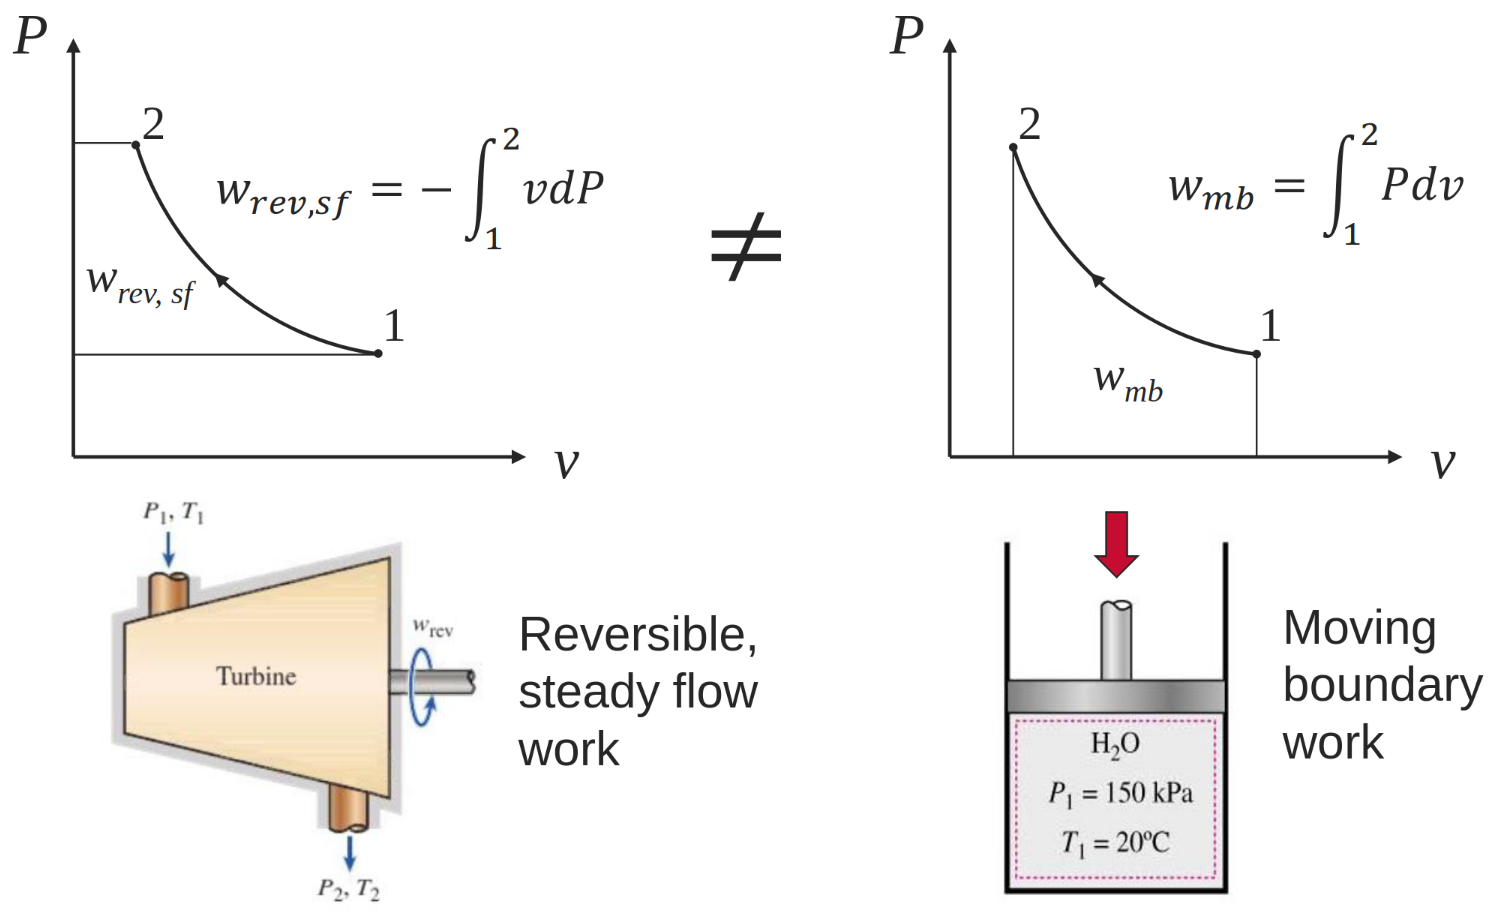
\includegraphics[width=.9\linewidth]{./images/reversible-steady-flow-work.png}
\end{center}

\subsubsection{Incompressible fluids}
\label{sec:org7b4468d}
\begin{itemize}
\item For incompressible fluids (constant specific volume \(v\)) and \(\Delta KE = 0\) and \(\Delta PE = 0\), like pumps:
\[w_{rev} = -v (P_2 - P_1)\]
\item In flow devices where it does \textbf{no work} and the fluid is \textbf{incompressible} (e.g. nozzles or pipes), use the Bernoulli equation
\[0 = -v (P_2 - P_1) - \frac{\nu_2^2 - \nu_1^2}{2} - g(z_2 - z_1)\]
\end{itemize}

\subsubsection{Fluid types}
\label{sec:orgb4afd03}
\begin{itemize}
\item Examining:
\[w_{rev} = - \int_1^2 v \, dP\]
\item Reversible steady flow work is closely associated to the specific volume \(v\) of the fluid flow through the device. The larger the specific volume, the larger the work produced or consumed.
\item Pumps handle liquids (small specific volume) and hence consumes less power.
\item Compressors handle gases (large specific volume) and tends to consume more power.
\end{itemize}

 \newpage

\subsection{Polytropic work in steady flow devices [formula given]}
\label{sec:org86bcf87}
\begin{itemize}
\item For a \textbf{polytropic process}:
\[Pv^n = \text{constant}\]
\item Work done when \textbf{flow} through the device is \textbf{polytropic}:
\begin{align*}
w_{poly} = \int_1^2 v \, dP &= - \int_1^2 \left(\frac{C}{P} \right)^{\frac{1}{n}} dP
&= - \frac{n}{n - 1}(P_2 v_2 - P_1 v_1)
\end{align*}
\item Not to be confused with polytropic work in a \textbf{closed system}:
\[w_{poly} = \int_1^2 P \, dv = - \frac{1}{n - 1} (P_2 v_2 - P_1 v_1)\]
\item For an \textbf{ideal gas}:
\[Pv = R_{sp} T\]
\[w_{poly} = - \frac{n R_{sp} (T_2 - T_1)}{n - 1} = - \frac{n R_{sp} T_1}{n - 1} \left[\left(\frac{P_2}{P_1} \right)^{\frac{n - 1}{n}} - 1 \right]\]
\end{itemize}

\subsubsection{Isentropic process for ideal gas}
\label{sec:orgca3eefc}
When the process is isentropic:
\[n = k\]
\[w_{isen} = - \frac{k R_{sp} (T_2 - T_1)}{k - 1} = \frac{k R_{sp} T_1}{1 - k} \left[\left(\frac{P_2}{P_1} \right)^{\frac{k - 1}{k}} - 1 \right]\]

\subsubsection{Isothermal process}
\label{sec:orgf17f289}
A gas undergoing unrestrained expansion is an isothermal process.

When the process is isothermal:
\[n = 1\]
\[w_{\text{isothermal}} = - R_{sp} T \ln \left(\frac{P_2}{P_1} \right)\]

\subsubsection{Minimum compressor work}
\label{sec:org09ce219}
\begin{itemize}
\item When compressing an ideal gas between the same pressure ratio, cooling the gas helps reduce the power consumption.
\item Multistage compression with inter-cooling:
\begin{center}
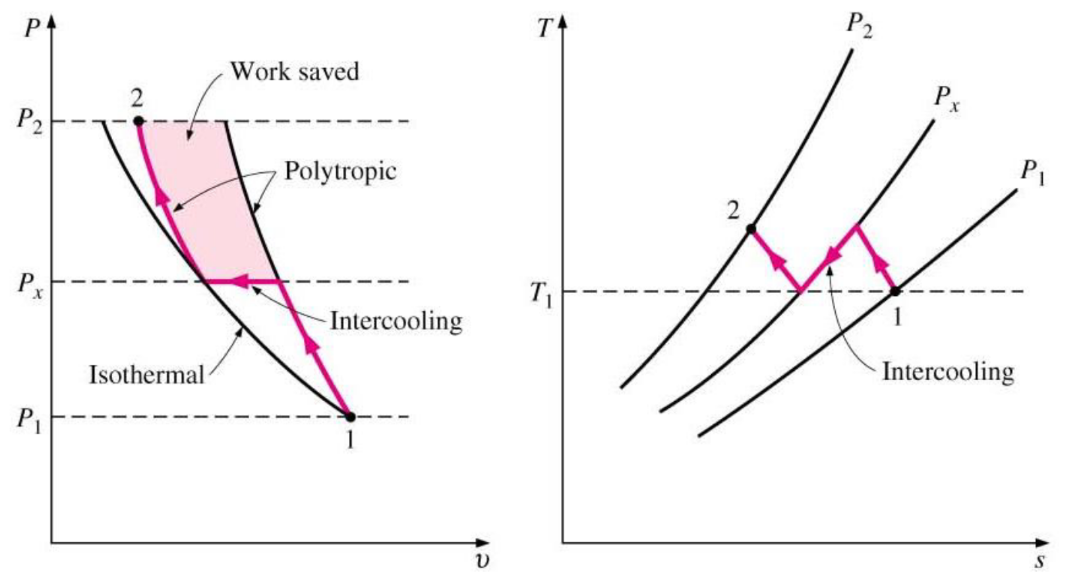
\includegraphics[width=.9\linewidth]{./images/multistage-compression-with-inter-cooling.png}
\end{center}
\item Work in two-stage compression with inter-cooling:
\[w_{comp} = w_{comp_1} + w_{comp_2} = - \frac{n R_{sp} T_1}{n - 1} \left[\left(\frac{P_x}{P_1} \right)^{\frac{n - 1}{n}} - 1 \right] - \frac{n R_{sp} T_1}{n - 1} \left[\left(\frac{P_2}{P_x} \right)^{\frac{n - 1}{n}} - 1 \right]\]
\item Minimum total work is when \textbf{pressure ratio} across each stage is the \textbf{same}:
\[P_x = \sqrt{P_1 P_2} \Rightarrow \frac{P_x}{P_1} = \frac{P_2}{P_x}\]
\end{itemize}

 \newpage

\subsection{Steady state control volume}
\label{sec:orgfc8189c}
\begin{itemize}
\item Many steady state control volume devices are \textbf{adiabatic} or \textbf{close to adiabatic} during operation.
\item Such devices work \textbf{best when irreversibilities are minimised}.
\item \textbf{Isentropic processes} would serve as the \textbf{ideal models} for these devices.
\begin{itemize}
\item Turbines, which extract work from the fluid, decreases the enthalpy of the fluid.
\item Pumps and compressors, which do work on the fluid, increases the enthalpy of the fluid.
\item Nozzles, which accelerate the fluid, decreases the enthalpy but increases the kinetic energy of the fluid. There is no work done for a nozzle.
\end{itemize}
\item \textbf{Isentropic processes} would serve as the \textbf{ideal process} for such \textbf{adiabatic} steady flow devices.
\item \textbf{Isentropic efficiencies} of turbines, compressors and pumps, and nozzles serve to compare the actual performance of these (\textbf{adiabatic}) devices to isentropic conditions at the \textbf{same inlet state} and \textbf{exit pressure}.
\end{itemize}

\begin{center}
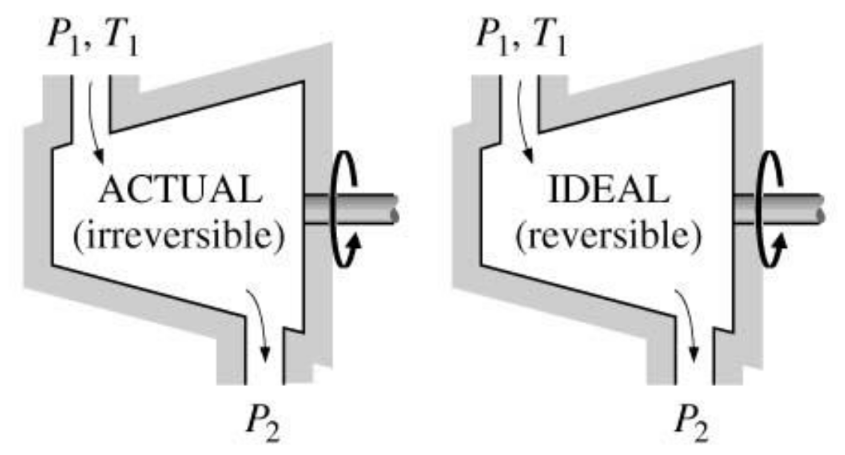
\includegraphics[width=.9\linewidth]{./images/isentropic-efficiency-comparison.png}
\end{center}

\subsection{Isentropic efficiency}
\label{sec:org3aaef8b}
Isentropic efficiency is the measure of the \textbf{deviation} of the \textbf{actual} (adiabatic) process from the \textbf{idealised} one.

\subsubsection{Figuring out the isentropic efficiency formula}
\label{sec:org4cb8a61}
\begin{enumerate}
\item Draw a \(h-s\) diagram.
\item Draw 2 pressure lines, one representing the initial pressure, and one representing the final pressure.
\item Draw one vertical connecting the two pressure lines to represent the isentropic process.
\item Draw a line that curves to the right connecting the two pressure lines to represent the actual process.
\item To get the efficiency, take the smaller change in enthalpy over the larger change in enthalpy.
\end{enumerate}

 \newpage

\subsubsection{Turbines}
\label{sec:org1af7c45}
\[w_T = h_1 - h_2\]
\[\eta_T = \frac{\text{Actual work}}{\text{Isentropic work}} = \frac{w_a}{w_s}\]
\[\eta_T = \frac{h_1 - h_{2a}}{h_1 - h_{2s}}\]

\begin{itemize}
\item \(\eta_T\) is roughly 90\% for large turbines
\item \(\eta_T\) is roughly 70\% for small turbines
\end{itemize}

\begin{center}
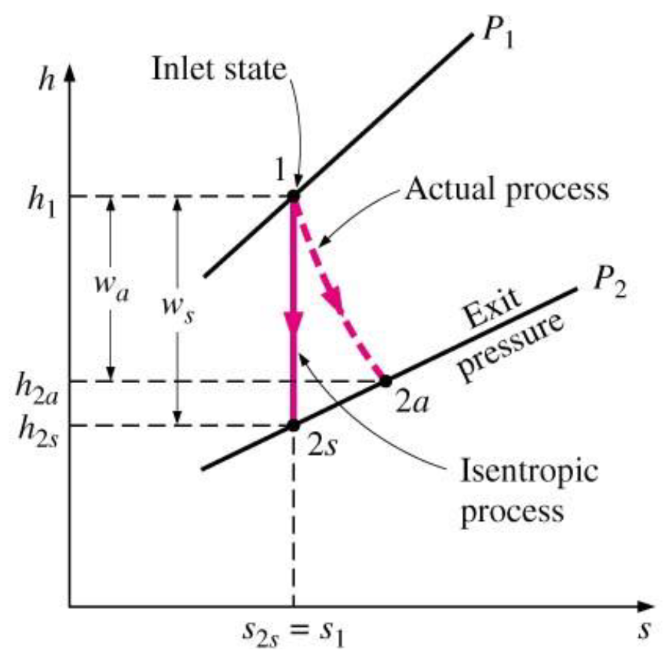
\includegraphics[scale=0.75]{./images/isentropic-efficiency-of-turbines.png}
\end{center}

Where:
\begin{itemize}
\item \(w_T\) is the work done by the turbine
\item \(\eta_T\) is the isentropic efficiency of the turbine
\item \(w_s\) is the isentropic work output of the turbine
\item \(w_a\) is the actual work output of the turbine
\item \(h_1\) is the initial enthalpy of the fluid
\item \(h_{2a}\) is the final enthalpy of the actual process
\item \(h_{2s}\) is the final enthalpy of the isentropic process
\end{itemize}

\subsubsection{Compressors}
\label{sec:orga188627}
\[w_C = -(h_1 - h_2)\]
\[\eta_C = \frac{\text{Isentropic work}}{\text{Actual work}} = \frac{w_s}{w_a}\]
\[\eta_T = \frac{h_{2s} - h_1}{h_{2a} - h_1}\]

\begin{itemize}
\item \(\eta_C\) is roughly 75 - 85\% for well-designed devices
\end{itemize}

\begin{center}
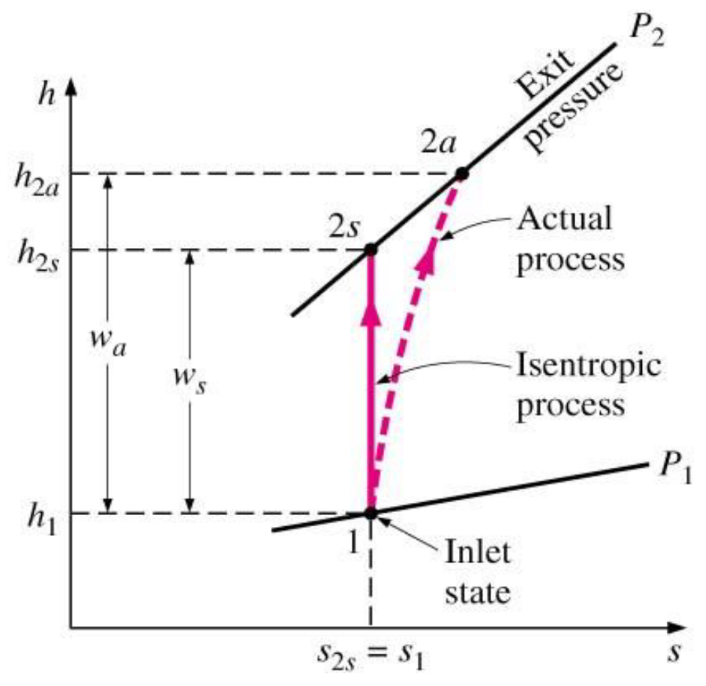
\includegraphics[scale=0.8]{./images/isentropic-efficiency-of-compressors.png}
\end{center}

Where:
\begin{itemize}
\item \(w_C\) is the work required by the compressor
\item \(\eta_C\) is the isentropic efficiency of the compressor
\item \(w_s\) is the isentropic work input into the compressor
\item \(w_a\) is the actual work input into the compressor
\item \(h_{2a}\) is the final enthalpy of the actual process
\item \(h_{2s}\) is the final enthalpy of the isentropic process
\item \(h_1\) is the initial enthalpy of the fluid
\end{itemize}

\subsubsection{Pumps}
\label{sec:org9485068}
\[w_{rev} = - \int v \, dP\]
\[w_{on} = - \left(- \int v \, dP \right)\]
\[\eta_P = \frac{w_s}{w_a} = \frac{v \left(P_2 - P_1 \right)}{h_{2a} - h_1}\]

Where:
\begin{itemize}
\item \(w_{rev}\) is the work done by the fluid in the isentropic process
\item \(w_{on}\) is the work done on the fluid by the pump in the isentropic process
\item \(\eta_C\) is the isentropic efficiency of the pump
\item \(w_s\) is the isentropic work input of the pump
\item \(w_a\) is the actual work input of the pump
\item \(v\) is the specific volume of the fluid
\item \(P_2\) is the final pressure of the fluid
\item \(P_1\) is the initial pressure of the fluid
\item \(h_{2a}\) is the final enthalpy of the actual process
\item \(h_1\) is the initial enthalpy of the fluid
\end{itemize}

 \newpage

\subsubsection{Nozzles}
\label{sec:org9147f63}
\[\eta_N = \frac{\text{Actual KE at exit}}{\text{Isentropic KE at exit}} = \frac{\nu_{2a}^2}{\nu_{2s}^2}\]
\[h_1 - h_{2a} = \frac{\nu_{2a}^2}{2}\]
\[\eta_N = \frac{h_1 - h_{2a}}{h_1 - h_{2s}}\]

\begin{itemize}
\item Typical \(\eta_N\) is roughly 90 - 95\%
\end{itemize}

\begin{center}
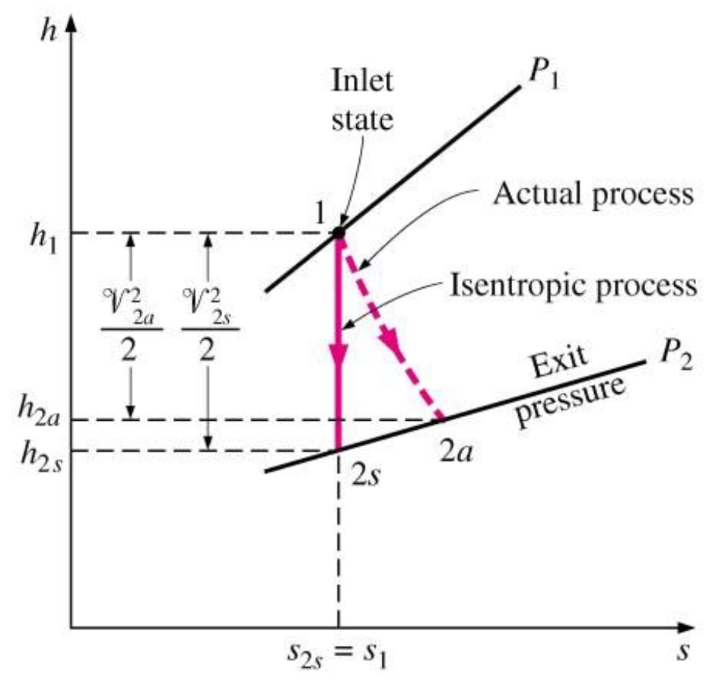
\includegraphics[scale=0.8]{./images/isentropic-efficiency-of-nozzles.png}
\end{center}

Where:
\begin{itemize}
\item \(\eta_N\) is the isentropic efficiency of the nozzle
\item \(\nu_{2a}\) is the final velocity of the actual process
\item \(\nu_{2s}\) is the final velocity of the isentropic process
\item \(h_{2a}\) is the final enthalpy of the actual process
\item \(h_{2s}\) is the final enthalpy of the isentropic process
\item \(h_1\) is the initial enthalpy of the fluid
\end{itemize}

\subsection{Gravimetric analysis}
\label{sec:org1d27df4}
The total mass of a mixture is equal to the sum of the mass of each component:
\[m_m = \sum_i^k m_i\]

\begin{center}
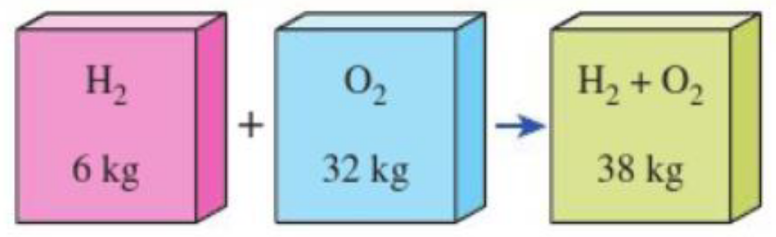
\includegraphics[width=.9\linewidth]{./images/gravimetric-analysis.png}
\end{center}

\subsubsection{Mass fraction}
\label{sec:org48dee89}
\begin{itemize}
\item Mass fraction is the ratio of mass of a component to the total mass of mixture:
\[mf_i = \frac{m_i}{m_m}\]
\item Sum of all mass fractions in the mixture is equal to 1:
\[\sum_i^k mf_i = 1\]
\end{itemize}

\subsection{Molar analysis}
\label{sec:org09a9094}
The total number of moles in a \textbf{non-reacting mixture} is equal to the sum of the number of moles of each component:
\[N_m = \sum_i^k N_i\]

\begin{center}
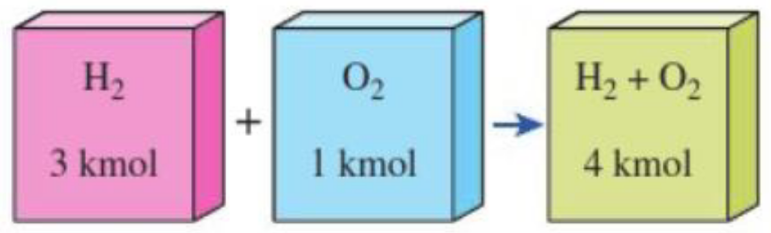
\includegraphics[width=.9\linewidth]{./images/molar-analysis.png}
\end{center}

\subsubsection{Mole fraction}
\label{sec:org935ac7e}
\begin{itemize}
\item Mole fraction is the ratio of the mole number of a component to the total mole number of the mixture:
\[y_i = \frac{N_i}{N_m}\]
\item Sum of all mole fractions in the mixture is equal to 1:
\[\sum_i^k y_i = 1\]
\end{itemize}

\subsection{Composition of gas mixtures}
\label{sec:org5be822d}
\begin{itemize}
\item Mass of substance \(m\) is equivalent to the product of its mole number \(N\) and molar mass \(M (m = NM)\).
\item Apparent (or average) molar mass of a mixture can be expressed as:
\begin{align*}
M_m &= \frac{m_m}{N_m} \\
&= \frac{\sum m_i}{N_m} \\
&= \frac{\sum N_i M_i}{N_m} \\
&= \sum_i^k y_i M_i
\end{align*}
\item Or:
\begin{align*}
M_m &= \frac{m_m}{N_m} \\
&= \frac{m_m}{\frac{\sum m_i}{M_i}} \\
&= \frac{1}{\frac{\sum m_i}{m_m M_i}} \\
&= \frac{1}{\sum_i^k \frac{mf_i}{M_i}}
\end{align*}
\item Gas constant for the mixture:
\[R_m = \frac{R_u}{M_m} \qquad R_u = \qty{8.314}{J.mol^{-1}.K^{-1}}\]
\end{itemize}

\subsection{Dalton's law of additive pressures}
\label{sec:org3650c60}
The pressure of a gas mixture is equal to the sum of the pressures each gas would exert if it existed alone at the mixture temperature and volume.

\begin{center}
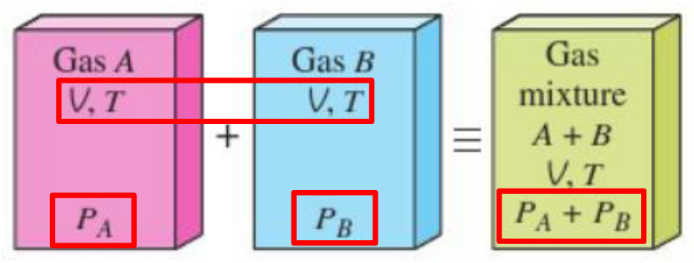
\includegraphics[width=.9\linewidth]{./images/daltons-law-of-additive-pressures.png}
\end{center}

\subsection{Amagat's law of additive volumes}
\label{sec:org334df83}
The volume of a gas mixture is equal to the sum of the volumes each gas would occupy if it existed alone at the mixture temperature and pressure.

\begin{center}
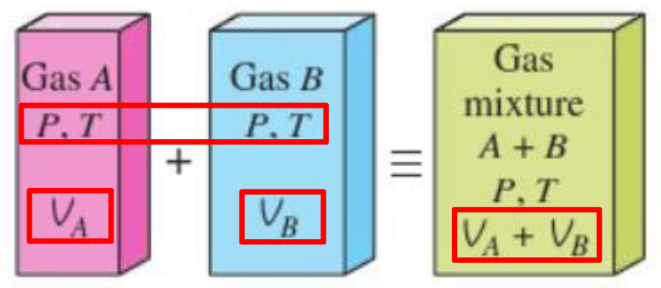
\includegraphics[width=.9\linewidth]{./images/amagats-law-of-additive-volumes.png}
\end{center}

 \newpage

\subsection{\(P-v-T\) behaviour of gas mixtures}
\label{sec:org7265e39}
\begin{itemize}
\item Dalton's and Amagat's laws hold \textbf{exactly} for \textbf{ideal-gas mixtures}.
\item The laws are \textbf{approximate} for \textbf{real-gas} mixtures, due to intermolecular forces which may be significant for real gases at high densities.
\item Dalton's law:
\[P_m = \sum_i^k P_i (T_m, V_m) \qquad P_i = \text{Component pressure}\]
\item Amagat's law:
\[V_m = \sum_i^k V_i (T_m, P_m) \qquad V_i = \text{Component volume}\]
\begin{itemize}
\item The component volume is the volume a component would occupy if it existed alone at \(T_m\) and \(P_m\), \textbf{not the actual volume} the component occupies \textbf{in the mixture}.
\begin{center}
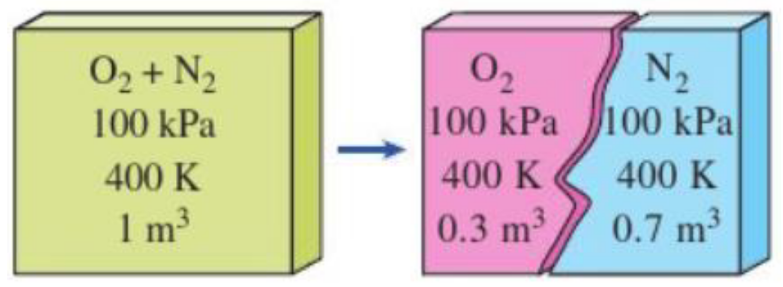
\includegraphics[width=.9\linewidth]{./images/component-volume-diagram.png}
\end{center}
\end{itemize}
\end{itemize}

 \newpage

\subsubsection{Ideal gases}
\label{sec:orgcffea23}
\begin{itemize}
\item Pressure fraction:
\[\frac{P_i(T_m, V_m)}{P_m} = \frac{\frac{(N_i R_u T_m)}{V_m}}{\frac{(N_m R_u T_m)}{V_m}} = \frac{N_i}{N_m} = y_i\]
\item The quantity \(y_i P_m\) is also called the partial pressure (component pressure for ideal gases).
\item Volume fraction:
\[\frac{V_i(T_m, P_m)}{V_m} = \frac{\frac{(N_i R_u T_m)}{P_m}}{\frac{(N_m R_u T_m)}{P_m}} = \frac{N_i}{N_m} = y_i\]
\item The quantity \(y_i V_m\) is also called the partial volume (component volume for ideal gases)
\item Dalton's law and Amagat's law are identical for ideal gases:
\[\frac{P_i}{P_m} = \frac{V_i}{V_m} = \frac{N_i}{N_m} = y_i\]
\end{itemize}

\subsection{Properties of gas mixtures}
\label{sec:org0721cd0}

\subsubsection{Extensive properties}
\label{sec:org340a55d}
\begin{displaymath}
\begin{array}{c|c}
\text{Extensive properties of gas mixtures} & \text{Changes in extensive properties of gas mixtures} \\
\hline
U_m = \sum_i^k U_i = \sum_i^k m_i u_i = \sum_i^k N_i \bar{u}_i &
\Delta U_m = \sum_i^k \Delta U_i = \sum_i^k m_i \Delta u_i = \sum_i^k N_i \Delta \bar{u}_i \\
H_m = \sum_i^k H_i = \sum_i^k m_i h_i = \sum_i^k N_i \bar{h}_i &
\Delta H_m = \sum_i^k \Delta H_i = \sum_i^k m_i \Delta h_i = \sum_i^k N_i \Delta \bar{h}_i \\
S_m = \sum_i^k S_i = \sum_i^k m_i s_i = \sum_i^k N_i \bar{s}_i &
\Delta S_m = \sum_i^k \Delta S_i = \sum_i^k m_i \Delta s_i = \sum_i^k N_i \Delta \bar{s}_i
\end{array}
\end{displaymath}

\subsubsection{Intensive properties}
\label{sec:org99e38fd}
Intensive properties of a mixture are determined by weighted averages.

\begin{displaymath}
\begin{array}{c|c}
u_m = \sum_i^k mf_i u_i & \bar{u}_m = \sum_i^k y_i \bar{u}_i \\
h_m = \sum_i^k mf_i h_i & \bar{h}_m = \sum_i^k y_i \bar{h}_i \\
s_m = \sum_i^k mf_i s_i & \bar{s}_m = \sum_i^k y_i \bar{s}_i \\
c_{v,m} = \sum_i^k mf_i c_{v,i} & \bar{c}_{v,m} = \sum_i^k y_i \bar{c}_{v,i} \\
c_{p,m} = \sum_i^k mf_i c_{p,i} & \bar{c}_{p,m} = \sum_i^k y_i \bar{c}_{p,i} \\
\end{array}
\end{displaymath}

\subsection{Dry and atmospheric air}
\label{sec:orgee04d3c}
\begin{itemize}
\item Air is a mixture of nitrogen, oxygen and small amounts of other gases.
\item Atmospheric air contains air and water vapour (moisture)
\begin{itemize}
\item Air and water vapour is atmospheric air
\item Air without water vapour is dry air
\end{itemize}
\item Water vapour (humidity) in the air affects human comfort, and hence is an important consideration for air-conditioning and heating applications
\item Water vapour in the air can be treated as an \textbf{ideal gas} (the error is less than 0.2\%) even when it is a saturated vapour.
\begin{itemize}
\item Atmospheric air can be treated as an ideal-gas mixture of air and water vapour.
\end{itemize}
\end{itemize}

\subsubsection{Properties}
\label{sec:orgcea3372}
\begin{itemize}
\item Dry air:
\[h_{\text{dry air}} = c_p T \qquad c_p = \qty{1.005}{kJ.kg^{-1}.\degreeCelsius^{-1}}\]

Use \(\qty{0}{\degreeCelsius}\) as the reference temperature, i.e.
\[\Delta h_{\text{dry air}} = c_p \Delta T\]

\item Pressure:
\[P = P_a + P_v\]

The total pressure is the sum of partial pressure of dry air (\(P_a\)) and the partial pressure of water vapour \(P_v\).

\item Water vapour:
\[h_v (T, \text{low } P) \cong h_g (T)\]
\[h_g (T) \cong 2500.9 + 1.82 T \qquad (\unit{kJ.kg^{-1}})\]

\begin{itemize}
\item The enthalpy of water vapour in atmospheric air can be taken to be equal to the enthalpy of \textbf{saturated vapour} at the \textbf{same temperature}.
\end{itemize}
\end{itemize}

\subsection{Humidity of air}
\label{sec:org0badd36}

\subsubsection{Specific or absolute humidity (\(\omega\))}
\label{sec:org62381b0}
Specific or absolute humidity is the ratio of mass of water vapour to the mass of dry air:
\[\omega = \frac{m_v}{m_a}\]

Alternatively:
\begin{align*}
\omega &= \frac{m_v}{m_a} \\
&= \frac{\frac{P_v V}{R_v T}}{\frac{P_a V}{R_a T}} \\
&= \frac{\frac{P_v}{R_v}}{\frac{P_a}{R_a}} \\
&= \frac{R_a}{R_v} \cdot \frac{P_v}{P_a} \\
&= 0.622 \frac{P_v}{P_a} \\
&= \frac{0.622 P_v}{P - P_v} \quad \because P = P_a + P_v
\end{align*}

No need to memorise this equation below, as it is given in the exam:
\[\frac{0.622 P_v}{P - P_v}\]

Specific humidity does not change with temperature unless condensation occurs.

\subsubsection{Saturated air}
\label{sec:orga8ae371}
\begin{itemize}
\item There is a \textbf{limit} to the amount of water vapour the air can hold.
\item At \textbf{maximum}, air is \textbf{saturated} with moisture (saturated air):
\[P_v = P_g \quad \text{where } P_g = P_{\text{sat @ T}}\]
\item Comfort level depends more on the \textbf{amount of moisture present} relative to the \textbf{maximum amount} that the air can hold at the same temperature.
\end{itemize}

\subsubsection{Relative humidity (\(\phi\))}
\label{sec:orgdad01a5}
Relative humidity is the ratio of moisture present to maximum amount that the air can hold.
\begin{align*}
\phi &= \frac{m_v}{m_g} \\
&= \frac{\frac{P_v V}{R_v T}}{\frac{P_g V}{R_v T}} \\
&= \frac{P_v}{P_g} \quad \text{where } P_g = P_{\text{sat @ T}}
\end{align*}

\begin{itemize}
\item Relative humidity changes with temperature since maximum moisture the air can hold depends on temperature.
\item Relative humidity ranges from 0 (dry air) to 1 (saturated air). The equations below are given in the exam:
\[\phi = \frac{\omega P}{(0.622 + \omega) P_g}\]
\[\omega = \frac{0.622 \phi P_g}{P - \phi P_g}\]
\item For practical applications, mass of dry air remains constant while the mass of water vapours can change.
\end{itemize}

\subsubsection{Intensive properties}
\label{sec:org6f39f39}
\begin{itemize}
\item Total enthalpy of atmospheric air:
\[H = H_a + H_v = m_a h_a + m_v h_v\]
\item Divide by mass of dry air (\(m_a\)):
\[h = \frac{H}{m_a} = h_a + \frac{m_v}{m_a} h_v = h_a + \omega h_v\]
\item Specific enthalpy of atmospheric air is expressed in terms of \textbf{per unit mass of dry air}:
\[h = h_a + \omega h_g \quad (\unit{kJ.kg^{-1}} \text{ dry air}) \quad \because h_v \cong h_g\]
\item Similarly, \textbf{specific volume} of atmospheric air is expressed in terms of per unit mass of dry air as well.
\[\text{Specific volume } (v): \unit{m^3.kg^{-1}} \text{ dry air}\]
\end{itemize}

\subsection{Dry-bulb temperature (\(T_{db}\))}
\label{sec:org93b1361}
Dry-bulb temperature is the normal temperature of atmospheric air.

\subsection{Dew point temperature (\(T_{dp}\))}
\label{sec:org90544d9}
Dew point temperature is the temperature at which condensation begins when air is cooled at constant pressure.
\begin{itemize}
\item Saturation temperature corresponding to the saturated vapour pressure.
\end{itemize}

\[T_{dp} = T_{\text{sat @ } P_v}\]

\begin{center}
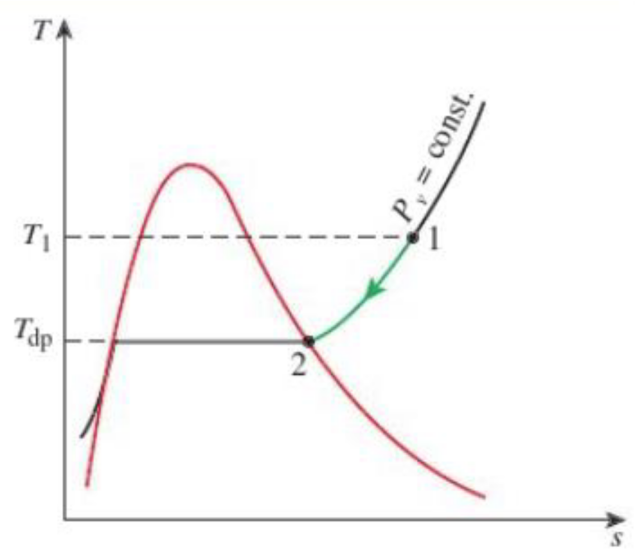
\includegraphics[width=.9\linewidth]{./images/dew-point-temperature-t-s-diagram.png}
\end{center}

 \newpage

\subsection{Adiabatic saturation process}
\label{sec:org819ebe4}
\begin{itemize}
\item Relative and specific humidity are important parameters in dealing with atmospheric air.
\item Calculation of relative and specific humidity can be achieved by measuring the dew point temperature, but this is not very practical.
\item Alternatively, relative and specific humidity can be related to an \textbf{adiabatic saturation process}.
\end{itemize}

\textbf{Diagrams:}

\begin{center}
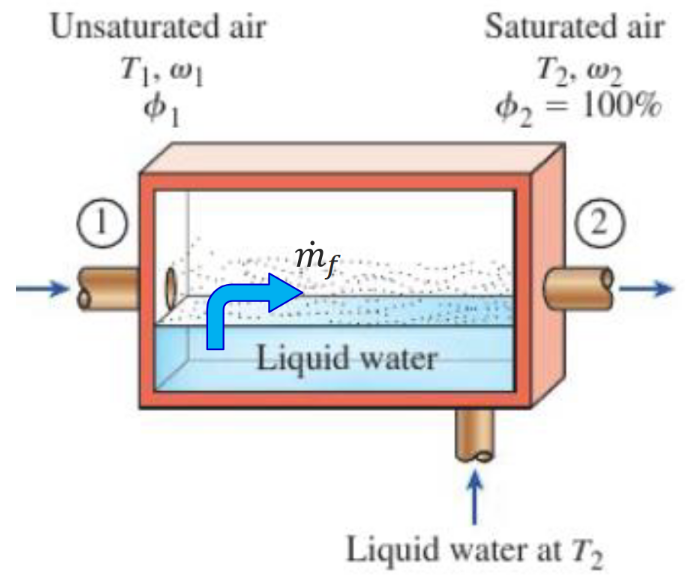
\includegraphics[scale=0.7]{./images/adiabatic-saturation-process-diagram.png}
\end{center}

\begin{center}
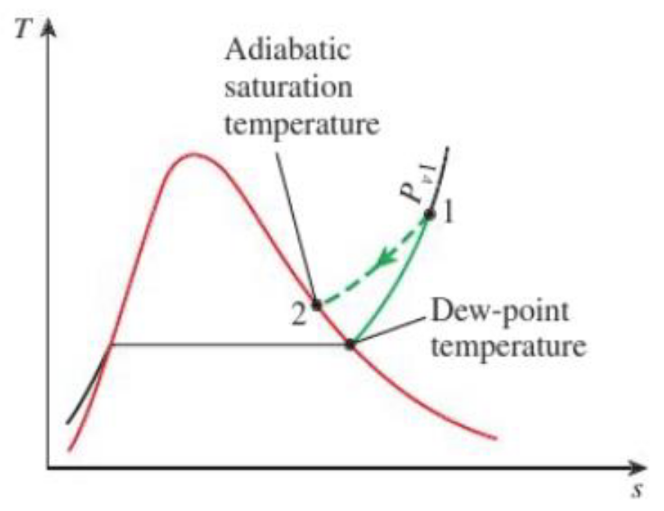
\includegraphics[scale=0.7]{./images/adiabatic-saturation-temperature-t-s-diagram.png}
\end{center}

\textbf{Details:}

\begin{itemize}
\item Assuming steady flow and negligible kinetic energy and potential energy.
\item Mass balance:
\[\dot{m}_{a_1} = \dot{m}_{a_2} = \dot{m_a} \quad (\text{Dry air})\]
\begin{displaymath}
\left. \begin{array}{c}
\dot{m}_{w_1} + \dot{m}_f = \dot{m}_{w2} \\
\omega_1 \dot{m}_{a_1} + \dot{m}_f = \omega_2 \dot{m}_{a_2} \\
\dot{m}_f = \dot{m}_a (\omega_2 - \omega_1)
\end{array} \right\} (\text{Water vapour})
\end{displaymath}

\(\dot{m}_f\) is the evaporation rate.

\item Energy balance: \(\dot{E}_{in} = \dot{E}_{out}\)
\[\dot{m}_a h_1 + \dot{m}_f h_{f_2} = \dot{m}_a h_2\]
\[\dot{m}_a h_1 + \dot{m}_a (\omega_2 - \omega_1) h_{f_2} = \dot{m}_a h_2\]
\[c_p T_1 + \omega_1 h_{g_1} + (\omega_2 - \omega_1) h_{f_2} = c_p T_2 + \omega_2 h_{g_2}\]

\item Rearrange for \(\omega_1\):
\[\omega_1 = \frac{c_p (T_2 - T_1) + \omega_2 h_{fg_2}}{h_{g_1} - h_{f_2}}\]
\begin{align*}
\omega_2 &= \frac{0.622 \phi_2 P_{g_2}}{P_2 - \phi_2 P_{g_2}} \qquad \text{when } \phi = 100\% \\
&= \frac{0.622 P_{g_2}}{P_2 - P_{g_2}}
\end{align*}

\item \(T_2\) is the adiabatic saturation temperature
\begin{itemize}
\item Process for determining \(T_2\) is still very impractical
\item Tank needs to be very long depending on the inlet specific humidity and requires perfect insulation and hence a more practical method is required.
\end{itemize}
\end{itemize}

\subsection{Wet-bulb temperature (\(T_{wb}\))}
\label{sec:org90f14ab}
\begin{itemize}
\item The wet-bulb temperature is the temperature measured using a thermometer whose bulb is covered with a cotton wick saturated with water and air blowing over the wick.
\item Wet-bulb temperature (\(T_{wb}\)) is \textbf{approximately equal} to adiabatic saturation temperature (\(T_2\)) at atmospheric pressures.
\[T_2 \cong T_{wb}\]
\item Water evaporating from the wick causes the temperature to drop, so:
\[T_{wb} < T_{dry}\]
\item At higher humidity, that means there is lower evaporation rate and hence a higher wet-bulb temperature.
\item When the wet-bulb temperature is equal to the temperature of dry air, the air is saturated with water, i.e.
\[T_{wb} = T_{dry} \quad \rightarrow \quad \phi = 100\%\]
\end{itemize}

\subsection{Specific volume of dry air}
\label{sec:org3db63f7}
\[v = \frac{P_a T}{R_a}\]

Where:
\begin{itemize}
\item \(v\) is the specific volume of dry air
\item \(P_a\) is the partial pressure of dry air
\item \(T\) is the temperature of the dry air in Kelvin
\item \(R_{a}\) is the molar gas constant per unit mass of dry air, which is \(\qty{0.287}{kJ.kg^{-1}.K^{-1}}\)
\end{itemize}

 \newpage

\subsection{Psychrometric chart}
\label{sec:orgfed41a8}
\begin{itemize}
\item The pressure value of the psychrometric chart below is \(\qty{1}{atm}\) or \(\qty{101.324}{kPa}\), which means it is only applicable this particular pressure value, which is at sea level.
\item The relative humidity lines are the lines that curve upwards from left to right. Note that the specific humidity values are on the inside of the \(y\)-axis, not outside. The values on the outside to the \(y\)-axis are enthalpy values.
\item The wet-bulb temperature line is the dotted lines parallel to the constant enthalpy lines, which are solid lines.
\item The dew point temperature lines are labelled on the saturation line, but can't be seen as they are blocked by the saturation line label.
\end{itemize}
\begin{center}
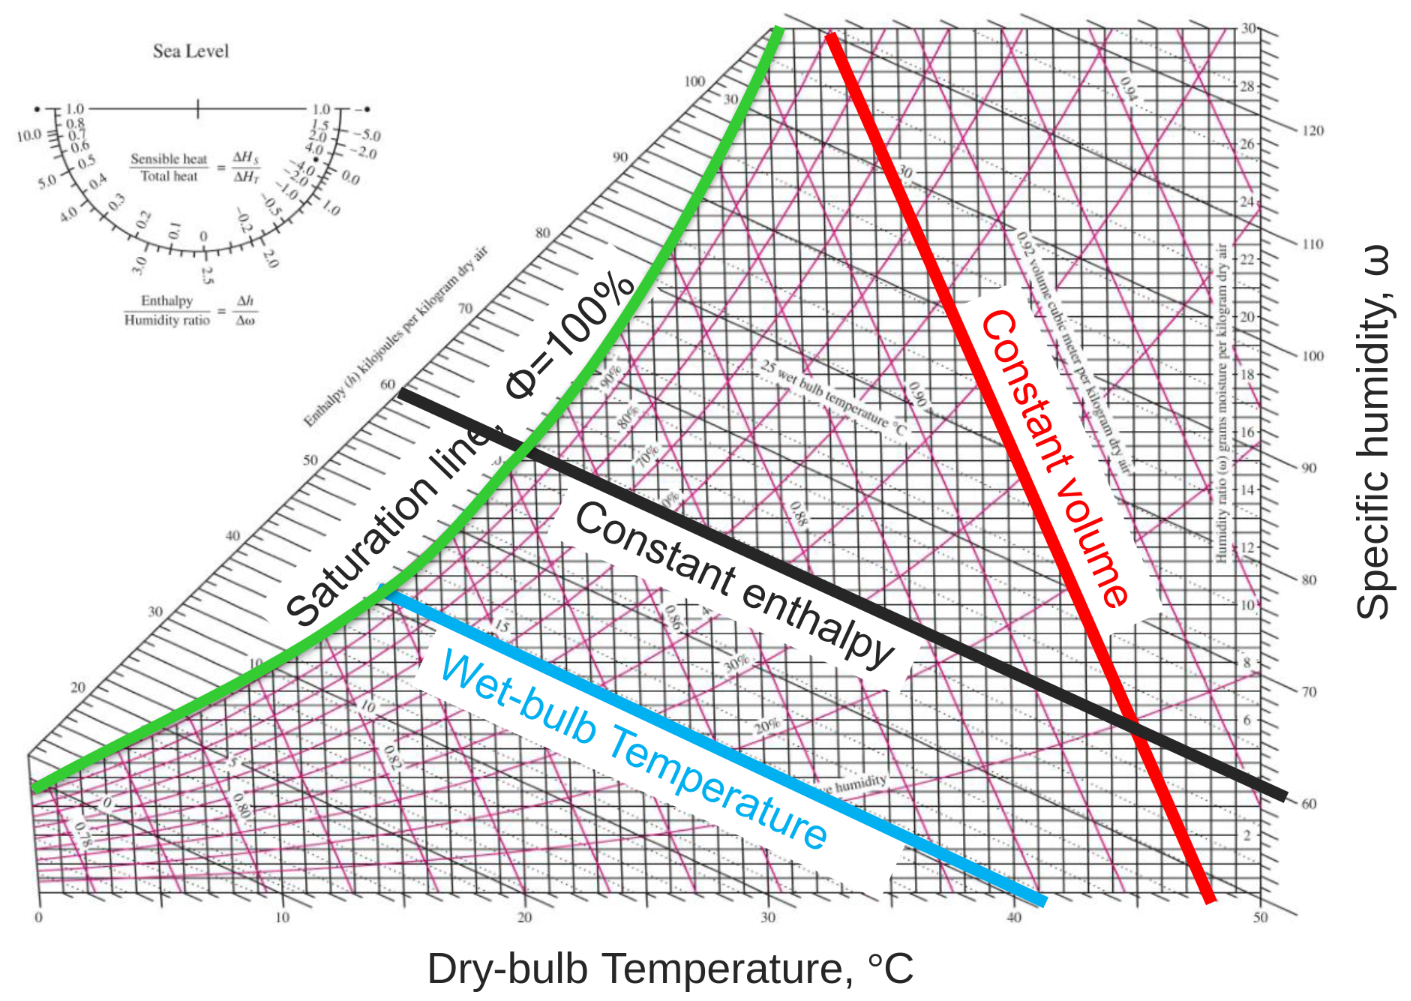
\includegraphics[width=.9\linewidth]{./images/psychrometric-chart.png}
\end{center}

\subsubsection{Schematic of the chart}
\label{sec:org5cdcf9a}
\begin{center}
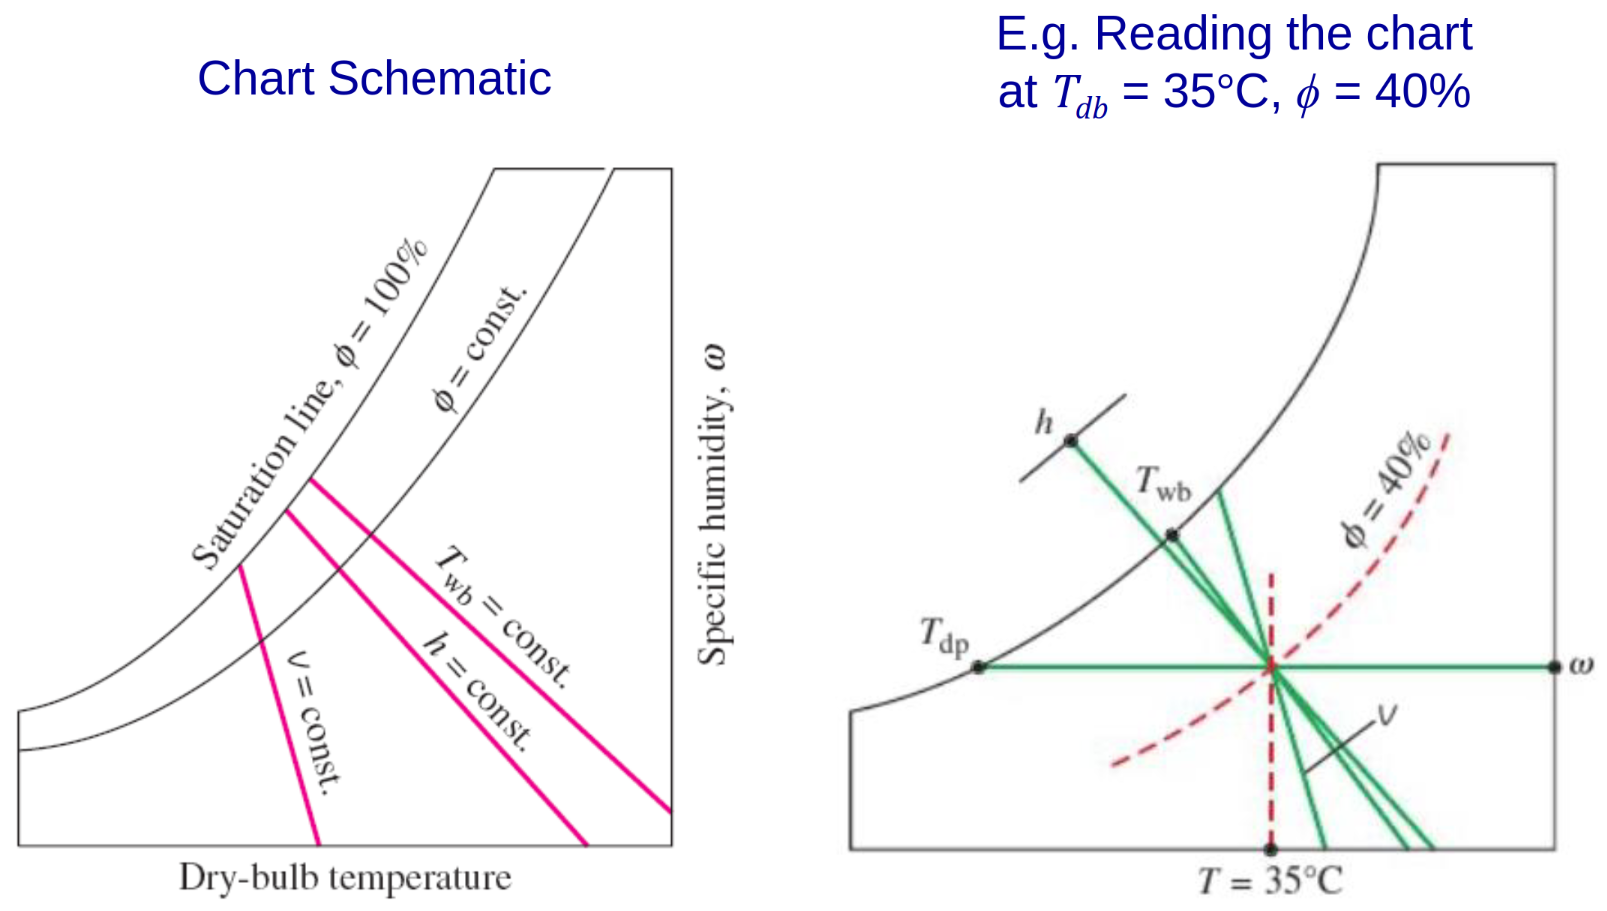
\includegraphics[width=.9\linewidth]{./images/psychrometric-chart-schematic.png}
\end{center}

\subsubsection{Example}
\label{sec:org7725b36}
\begin{center}
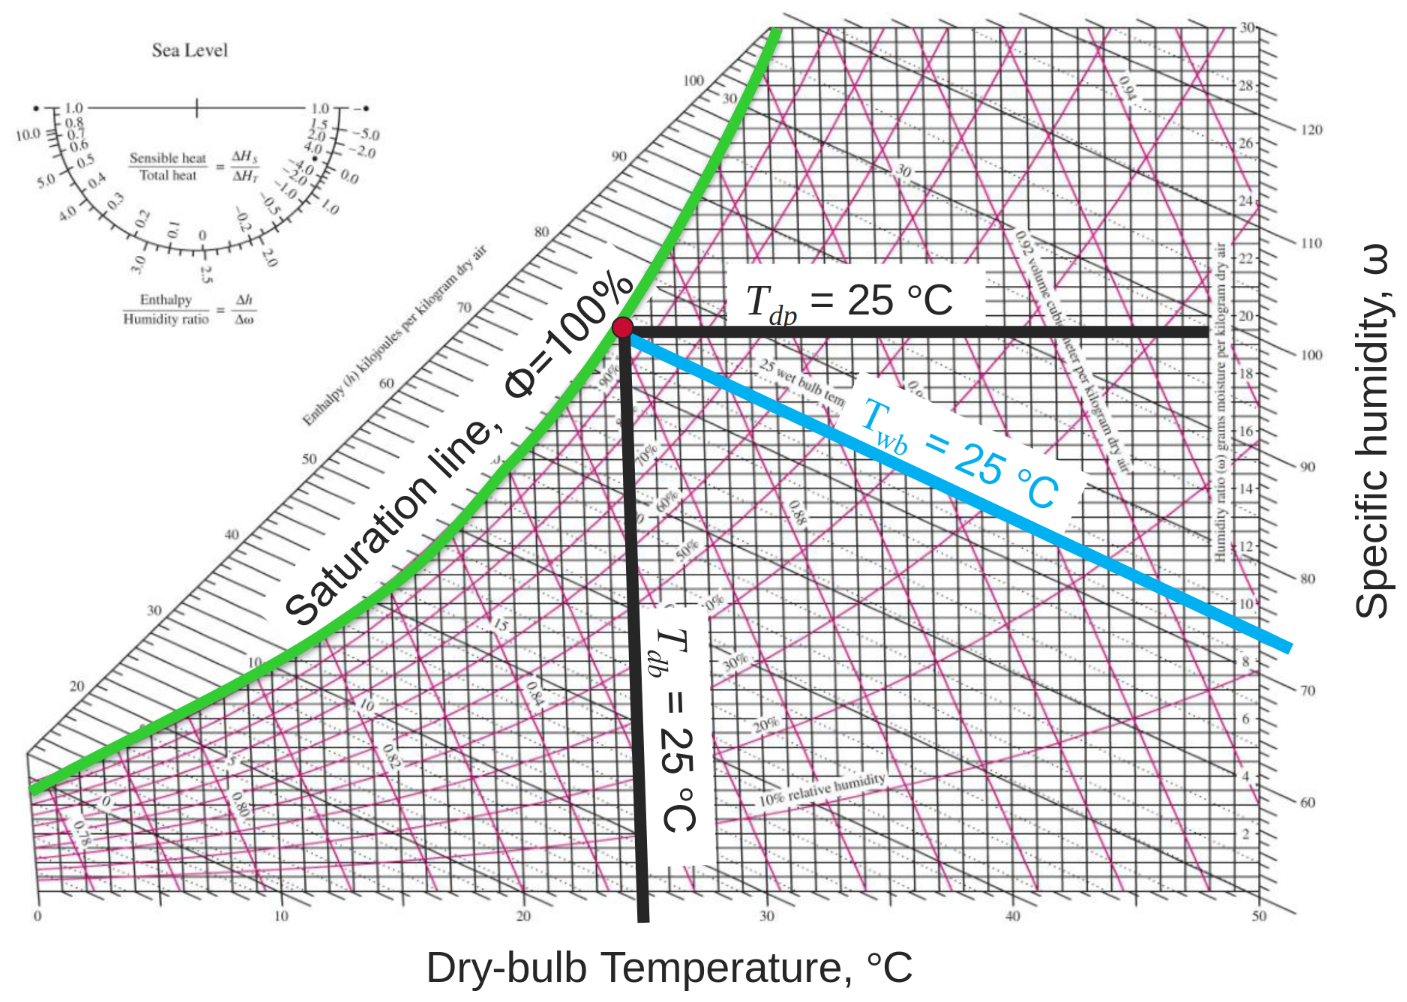
\includegraphics[width=.9\linewidth]{./images/psychrometric-chart-example.png}
\end{center}

For saturated air:
\[T_{db} = T_{wb} = T_{dp}\]

\subsection{Air conditioning processes}
\label{sec:orgdd782b6}
\begin{itemize}
\item Modern air-conditioning systems can heat, cool, humidify and dehumidify the air.
\item Modelling air-conditioning processes on the psychrometric chart:
\begin{center}
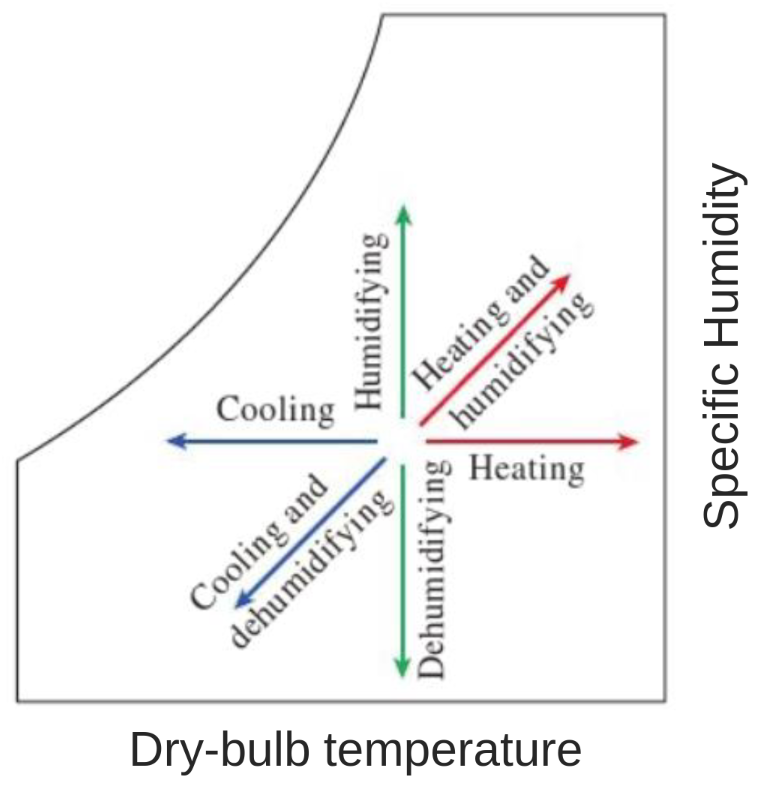
\includegraphics[scale=0.65]{./images/air-conditioning-processes-on-a-psychrometric-chart.png}
\end{center}
\item These processes are modelled as \textbf{steady flow} processes.
\item Kinetic energy and potential energy terms are ignored.
\item Mass balance: \(\sum_{in} \dot{m}_a = \sum_{out} \dot{m}_a\)
\[\text{Dry air:} \quad \sum_{in} \dot{m}_a = \sum_{out} \dot{m}_a\]
\[\text{Water:} \quad \sum_{in} \dot{m}_w = \sum_{out} \dot{m}_w \quad \rightarrow \quad \sum_{in} \omega \dot{m}_a = \sum_{out} \omega \dot{m}_a\]
\item Energy balance: \(\dot{E}_{in} = \dot{E}_{out}\)
\[\dot{Q}_{in} + \dot{W}_{in} + \sum_{in} \dot{m} h = \dot{Q}_{out} + \dot{W}_{out} + \sum_{out} \dot{m} h\]
\item Work term usually consists of \textbf{fan work input}, which is small relative to the other terms in the energy equation.
\end{itemize}

\subsubsection{Simple heating and cooling}
\label{sec:org1d2c812}
\begin{center}
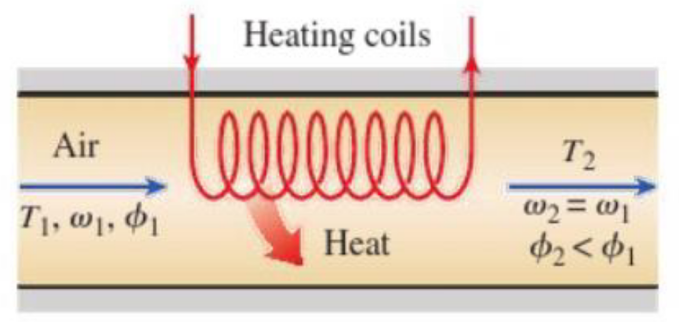
\includegraphics[scale=0.6]{./images/simple-heating-and-cooling-diagram.png}
\end{center}

\begin{center}
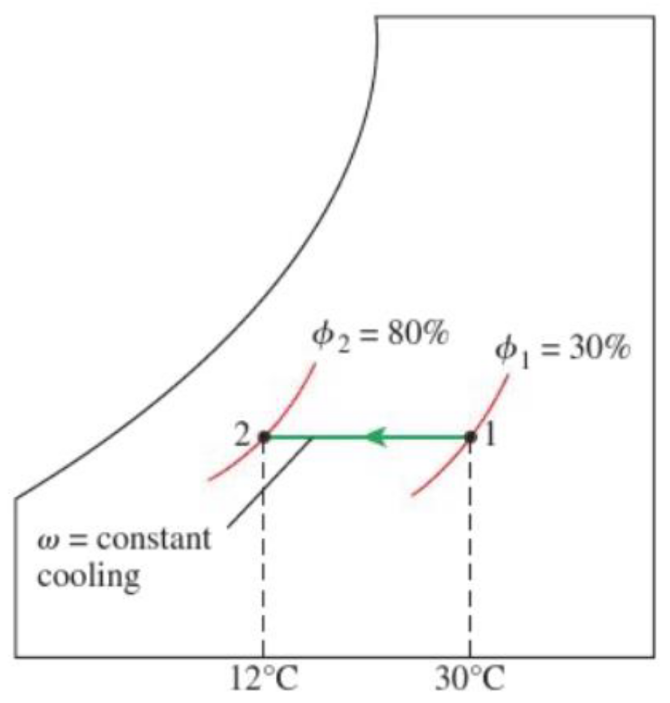
\includegraphics[scale=0.7]{./images/simple-heating-and-cooling-psychrometric-chart.png}
\end{center}
\begin{itemize}
\item Process appears as a horizontal line on the psychrometric chart
\item Specific humidity remains constant
\item Relative humidity decreases with heating
\item Relative humidity increases with cooling
\item Mass balance:
\[\dot{m}_{a_1} = \dot{m}_{a_2} = \dot{m}_a\]
\[\dot{m}_{w_1} = \dot{m}_{w_2} = \dot{m}_w \quad \rightarrow \quad \omega_1 = \omega_2\]
\item Energy balance:
\[\dot{Q} = \dot{m}_a (h_2 - h_1) \text{ or } q = (h_2 - h_1)\]
\end{itemize}

\subsubsection{Humidification or dehumidification}
\label{sec:org4c6f57c}
\[\dot{m}_w = \dot{m}_a \Delta \omega\]

Where:
\begin{itemize}
\item \(\dot{m}_w\) is the mass flow rate of water
\item \(\dot{m}_a\) is the mass flow rate of dry air
\item \(\Delta \omega\) is the change in specific humidity
\end{itemize}

\subsubsection{Heating with humidification}
\label{sec:org32d462a}
\textbf{Diagrams:}
\begin{center}
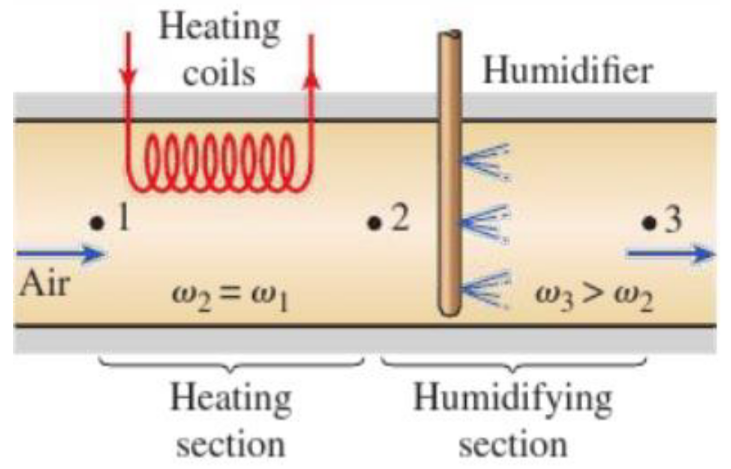
\includegraphics[scale=0.6]{./images/heating-with-humidification-diagram.png}
\end{center}

\begin{center}
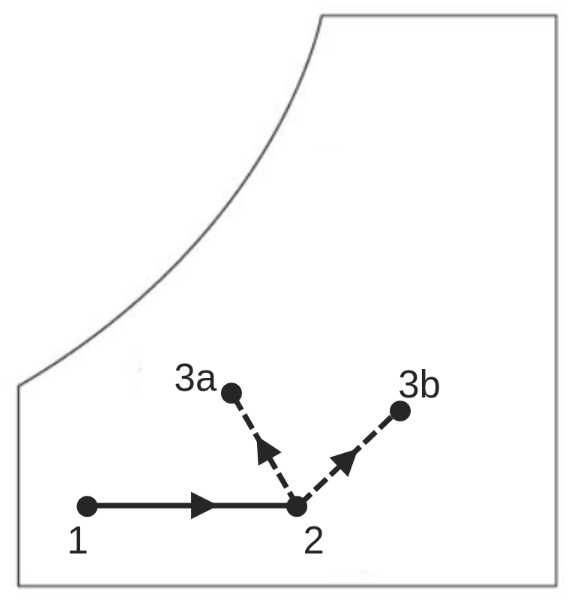
\includegraphics[scale=0.8]{./images/heating-with-humidification-psychrometric-chart.png}
\end{center}

\textbf{Details:}
\begin{itemize}
\item 2-step process:
\begin{enumerate}
\item Simple heating
\item Humidification
\end{enumerate}
\item Temperature after humidification depends on the process, for example:
\begin{enumerate}
\item Water spray: temperature decreases after humidification due to evaporation (a).
\item Steam spray: temperature increases (b).
\end{enumerate}
\item Simple heating (\(1 \rightarrow 2\)):
\[\dot{m}_{a_1} = \dot{m}_{a_2} = \dot{m}_a\]
\[\dot{m}_{w_1} = \dot{m}_{w_2} = \dot{m}_w \quad \rightarrow \quad \omega_1 = \omega_2\]
\[\dot{Q}_{in} = \dot{m}_a (h_2 - h_1)\]
\item Humidification (\(2 \rightarrow 3\)):
\[\omega_2 \dot{m}_{a_2} + \dot{m}_w = \omega_3 \dot{m}_{a_3}\]
\[\dot{m}_w = \dot{m}_a (\omega_3 - \omega_2)\]
\end{itemize}

 \newpage

\subsubsection{Cooling with dehumidification}
\label{sec:org73d1d4e}
\begin{center}
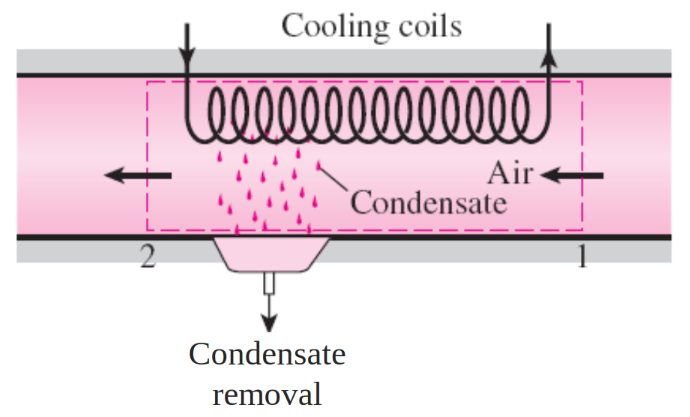
\includegraphics[scale=0.5]{./images/cooling-with-dehumidification-diagram.png}
\end{center}

\begin{center}
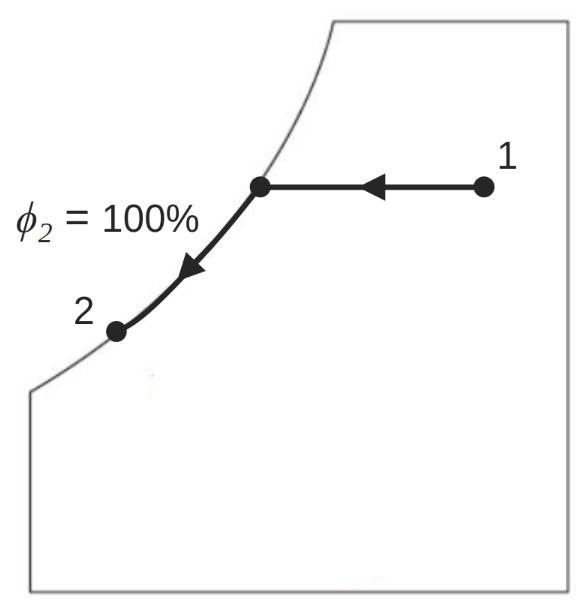
\includegraphics[scale=0.5]{./images/cooling-with-dehumidification-psychrometric-chart.png}
\end{center}
\begin{itemize}
\item Relative humidity increases with cooling, and eventually reaches 100\%
\item Cooling the air past the dew point temperature causes water vapour to condense. As condensed water (condensate) is removed, the air is dehumidified.
\item One-step process.
\item Mass balance:
\[\text{Dry air:} \quad \dot{m}_{a_1} = \dot{m}_{a_2} = \dot{m}_a\]
\[\text{Water:} \quad \dot{m}_{v_1} = \dot{m}_{v_2} + \dot{m}_w\]
\[\omega_1 \dot{m}_{a_1} = \omega_2 \dot{m}_{a_2} + \dot{m}_w\]
\[\dot{m}_w = \dot{m}_a (\omega_1 - \omega_2)\]
\item Energy balance:
\[\dot{Q}_{in} + \sum_{in} \dot{m} h = \dot{Q}_{out} + \sum_{out} \dot{m} h\]
\[\dot{m}_{a_1} h_1 = \dot{Q}_{out} + \dot{m}_{a_2} h_2 + \dot{m}_{w} h_w\]
\[\dot{Q}_{out} = \dot{m}_a (h_1 - h_2) - \dot{m}_w h_w\]
\end{itemize}

\subsubsection{Evaporative cooling}
\label{sec:org58f5641}
\begin{center}
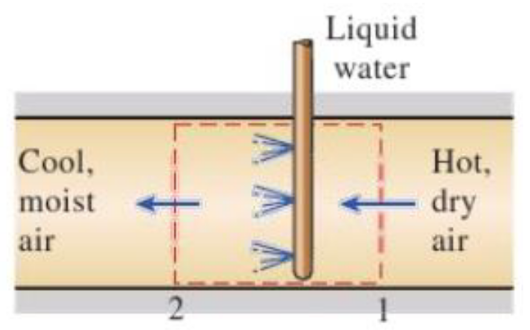
\includegraphics[scale=0.7]{./images/evaporative-cooling-diagram.png}
\end{center}

\begin{center}
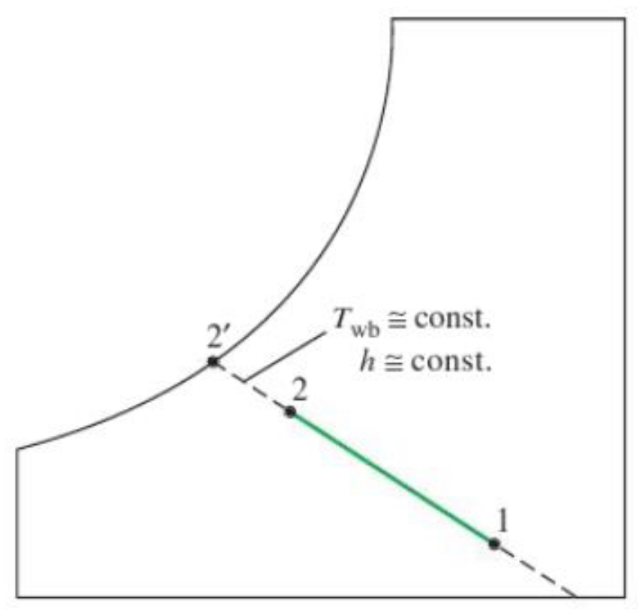
\includegraphics[scale=0.8]{./images/evaporative-cooling-psychrometric-chart.png}
\end{center}
\begin{itemize}
\item High cost of cooling is avoided by using evaporative coolers in the desert (hot and dry climates).
\item Evaporation of water cools the air and increases the humidity.
\item Evaporative cooling is identical to adiabatic saturation process.
\item Process follows constant wet-bulb temperature line.
\begin{itemize}
\item Enthalpy is also assumed to remain constant:
\[T_{wb} \cong \text{constant}\]
\[h \cong \text{constant}\]
\end{itemize}
\end{itemize}

\subsubsection{Adiabatic mixing of airstreams}
\label{sec:org6516f39}
\textbf{Diagrams:}
\begin{center}
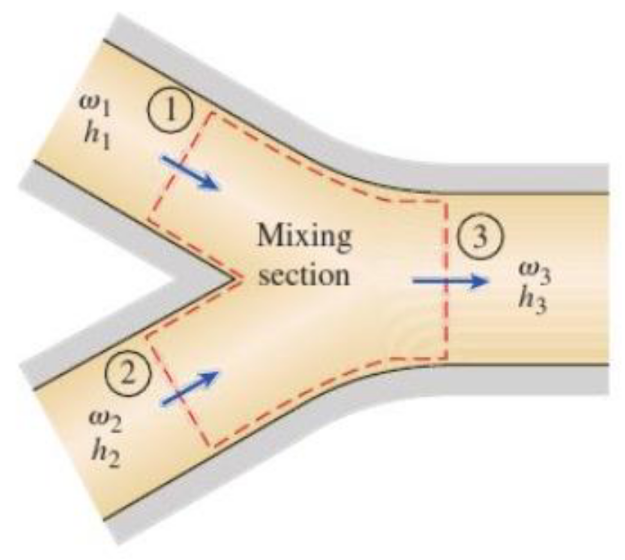
\includegraphics[scale=0.8]{./images/adiabatic-mixing-of-airstreams-diagram.png}
\end{center}

\begin{center}
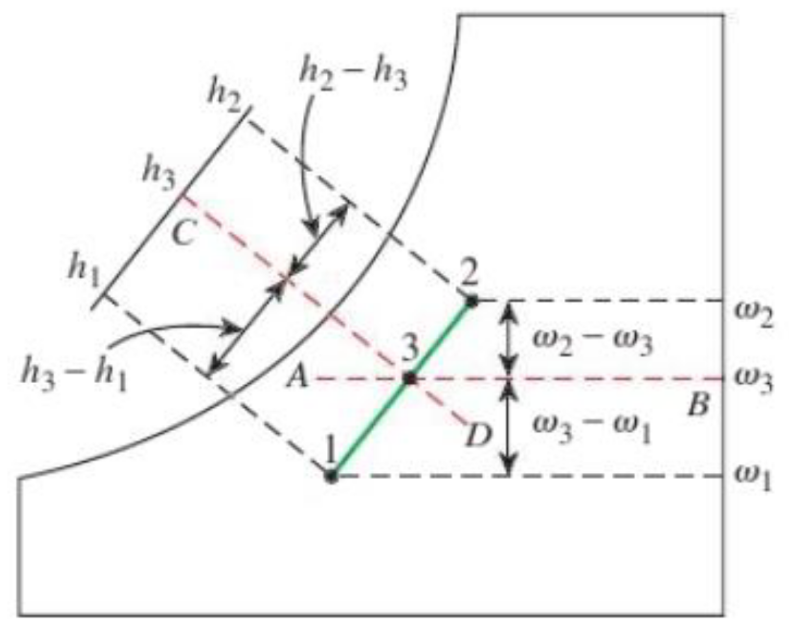
\includegraphics[scale=0.9]{./images/adiabatic-mixing-of-airstreams-psychrometric-chart.png}
\end{center}

\textbf{Details:}
\begin{itemize}
\item Mixing of airstreams is commonly used for air-conditioning in large buildings.
\item Heat transfer to the surroundings is usually small, so the process is \textbf{assumed to be adiabatic}.
\item Mass balance:
\[\text{Dry air:} \quad \dot{m}_{a_1} + \dot{m}_{a_2} = \dot{m}_{a_3}\]
\[\text{Water:} \quad \dot{m}_{w_1} + \dot{m}_{w_2} = \dot{m}_{v_3}\]
\[\omega_1 \dot{m}_{a_1} + \omega_2 \dot{m}_{a_2} = \omega_3 \dot{m}_{a_3}\]
\item Substituting and eliminating \(\dot{m}_{a_3}\):
\[\frac{\dot{m}_{a_1}}{\dot{m}_{a_2}} = \frac{\omega_2 - \omega_3}{\omega_3 - \omega_1}\]
\item Energy balance:
\[h_1 \dot{m}_{a_1} + h_2 \dot{m}_{a_2} = h_3 \dot{m}_{a_3}\]
\item Substituting and eliminating \(\dot{m}_{a_3}\):
\[\frac{\dot{m}_{a_1}}{\dot{m}_{a_2}} = \frac{h_2 - h_3}{h_3 - h_1} = \frac{\omega_2 - \omega_3}{\omega_3 - \omega_1}\]
\item Equation is in the form of a geometric interpolation.
\item When two airstreams at states 1 and 2 are mixed adiabatically, the state of the mixture lies in the straight line connecting the two states.
\end{itemize}

 \newpage

\section{Formulas}
\label{sec:org0b83f22}

\subsection{Change in specific internal energy of an ideal gas}
\label{sec:org4598693}
\[\Delta u = c_{\text{v, avg}} (T_2 - T_1)\]

Where:
\begin{itemize}
\item \(\Delta u\) is the change in specific internal energy of an ideal gas
\item \(c_{\text{v, avg}}\) is the specific heat capacity of the ideal gas at constant volume
\item \(T_2\) is the final temperature
\item \(T_1\) is the initial temperature
\end{itemize}

\subsection{Change in specific enthalpy of an ideal gas}
\label{sec:orgee5e389}
\[\Delta h = c_{\text{p, avg}} (T_2 - T_1)\]

Where:
\begin{itemize}
\item \(\Delta u\) is the change in specific enthalpy of an ideal gas
\item \(c_{\text{p, avg}}\) is the specific heat capacity of the ideal gas at constant pressure
\item \(T_2\) is the final temperature
\item \(T_1\) is the initial temperature
\end{itemize}

\subsection{Quality (dryness fraction) (\(x\))}
\label{sec:org7707bf3}
\[x = \frac{m_{vapour}}{m_{total}} = \frac{m_g}{m_f + m_g}\]

Where:
\begin{itemize}
\item \(x\) is the quality or dryness fraction
\item \(m_{vapour}\) is the mass of vapour
\item \(m_{total}\) is the total mass
\item \(m_g\) is the mass of vapour
\item \(m_f\) is the mass of liquid
\end{itemize}

\subsubsection{Specific entropy in terms of quality (\(s\))}
\label{sec:org8036bda}
\[s = s_f + xs_{fg}\]

Where:
\begin{itemize}
\item \(s\) is the specific entropy
\item \(s_f\) is the specific entropy of the saturated liquid
\item \(s_g\) is the specific entropy of the saturated vapour
\item \(s_{fg}\) is the specific entropy of the mixture at evaporation, where \(s_{fg} = s_g - s_f\)
\end{itemize}

\subsubsection{Quality in terms of specific entropy (\(x\))}
\label{sec:orgba9b6f8}
\[x = \frac{s - s_f}{s_{fg}}\]

Where:
\begin{itemize}
\item \(x\) is the quality
\item \(s\) is the specific entropy of the mixture
\item \(s_f\) is the specific entropy of the saturated liquid
\item \(s_g\) is the specific entropy of the saturated vapour
\item \(s_{fg}\) is the specific entropy of the mixture at evaporation, where \(s_{fg} = s_g - s_f\)
\end{itemize}

\subsection{Net work output of a heat engine}
\label{sec:org8350437}
\[W_{\text{net, out}} = W_{out} - W_{in}\]

Where:
\begin{itemize}
\item \(W_{\text{net, out}}\) is the net work output of the heat engine
\item \(W_{out}\) is the work done \textbf{by} the heat engine
\item \(W_{in}\) is the work done \textbf{on} the heat engine
\end{itemize}

\subsection{Energy balance of a heat engine}
\label{sec:org986e950}
\[W_{\text{net, out}} = Q_{in} - Q_{out}\]

Where:
\begin{itemize}
\item \(W_{\text{net, out}}\) is the net work output of the heat engine
\item \(Q_{in}\) is the heat energy input from the high temperature reservoir
\item \(Q_{out}\) is the heat energy output from the low temperature reservoir
\end{itemize}

\subsection{Thermal efficiency}
\label{sec:org4c36e52}
\[\text{Thermal efficiency} = \frac{\text{Desired output}}{\text{Required input}}\]

\subsubsection{Heat engine}
\label{sec:org72994ab}
\[\eta_{th} = \frac{W_{\text{net, out}}}{Q_{H}} = 1 - \frac{Q_L}{Q_H}\]

Where:
\begin{itemize}
\item \(\eta_{th}\) is the efficiency of the heat engine
\item \(W_{\text{net, out}}\) is the net work output of the heat engine
\item \(Q_{H}\) is the heat energy transferred from the high temperature reservoir (\(H\) for high temperature)
\item \(Q_{L}\) is the heat energy transferred from the low temperature reservoir (\(L\) for low temperature)
\end{itemize}

\subsubsection{Carnot heat engine}
\label{sec:orga85be6d}
\[\eta_{\text{th, rev}} = 1 - \frac{T_L}{T_H}\]

Where:
\begin{itemize}
\item \(\eta_{th}\) is the efficiency of a Carnot heat engine
\item \(T_{H}\) is the temperature of the high temperature reservoir (\(H\) for high temperature)
\item \(T_{L}\) is the temperature of the low temperature reservoir (\(L\) for low temperature)
\end{itemize}

\subsection{Energy balance of a reverse heat engine (refrigerators and heat pumps)}
\label{sec:org8807ff6}
\[W_{\text{net, in}} = Q_{H} - Q_{L}\]

Where:
\begin{itemize}
\item \(W_{\text{net, in}}\) is the net energy input into the reverse heat engine
\item \(Q_{H}\) is the heat energy transferred from the high temperature reservoir (\(H\) for high temperature)
\item \(Q_{L}\) is the heat energy transferred from the low temperature reservoir (\(L\) for low temperature)
\end{itemize}

\subsection{Coefficient of performance}
\label{sec:orgaec6502}
\[\text{Coefficient of performance} = \frac{\text{Desired output}}{\text{Required input}}\]

\subsubsection{Refrigerator}
\label{sec:org2344469}
\[COP_R = \frac{Q_L}{Q_H - Q_L} = \frac{1}{\frac{Q_H}{Q_L} - 1}\]

Where:
\begin{itemize}
\item \(COP_R\) is the coefficient of performance of the refrigerator
\item \(Q_{H}\) is the heat energy transferred from the high temperature reservoir (\(H\) for high temperature)
\item \(Q_{L}\) is the heat energy transferred from the low temperature reservoir (\(L\) for low temperature)
\end{itemize}

\subsubsection{Carnot refrigerator}
\label{sec:org5c6d5ce}
\[COP_{\text{R, rev}} = \frac{T_L}{T_H - T_L} = \frac{1}{\frac{T_H}{T_L} - 1}\]

Where:
\begin{itemize}
\item \(COP_{\text{R, rev}}\) is the coefficient of performance of a Carnot refrigerator
\item \(T_{H}\) is the temperature of the high temperature reservoir (\(H\) for high temperature)
\item \(T_{L}\) is the temperature of the low temperature reservoir (\(L\) for low temperature)
\end{itemize}

\subsubsection{Heat pump}
\label{sec:org614903b}
\[COP_{HP} = \frac{Q_H}{Q_H - Q_L} = \frac{1}{1 - \frac{Q_L}{Q_H}}\]

Where:
\begin{itemize}
\item \(COP_{HP}\) is the coefficient of performance of the heat pump
\item \(Q_{H}\) is the heat energy transferred from the high temperature reservoir (\(H\) for high temperature)
\item \(Q_{L}\) is the heat energy transferred from the low temperature reservoir (\(L\) for low temperature)
\end{itemize}

\subsubsection{Carnot heat pump}
\label{sec:org7bc41b3}
\[COP_{\text{HP, rev}} = \frac{Q_H}{Q_H - Q_L} = \frac{1}{1 - \frac{Q_L}{Q_H}}\]

Where:
\begin{itemize}
\item \(COP_{\text{HP, rev}}\) is the coefficient of performance of a Carnot heat pump
\item \(T_{H}\) is the temperature of the high temperature reservoir (\(H\) for high temperature)
\item \(T_{L}\) is the temperature of the low temperature reservoir (\(L\) for low temperature)
\end{itemize}

 \newpage

\subsection{Clausius Inequality}
\label{sec:org539568d}
\[\oint \frac{\delta Q}{T} \leq 0\]

For reversible cycles:
\[\oint \frac{\delta Q}{T} = 0\]

For irreversible cycles:
\[\oint \frac{\delta Q}{T} < 0\]

Where:
\begin{itemize}
\item \(\delta Q\) is an infinitesimal amount of heat that is taken from the reservoirs and absorbed by the system. \(\delta Q > 0\) if heat from the reservoirs is absorbed by the system, and \(\delta Q < 0\) is heat is leaving from the system to the reservoirs.
\item \(T\) is the common temperature of the reservoirs at a particular instant in time in Kelvin
\end{itemize}

\subsection{Entropy}
\label{sec:org11c9b71}
\[dS = \left(\frac{\delta Q}{T} \right)_{\text{int rev}} \quad \left(\unit{kJ.K^{-1}}\right)\]

Where:
\begin{itemize}
\item \(dS\) is the change in entropy for an internally reversible process (int rev)
\item \(\delta Q\) is an infinitesimal amount of heat that is taken from the reservoirs and absorbed by the system. \(\delta Q > 0\) if heat from the reservoirs is absorbed by the system, and \(\delta Q < 0\) is heat is leaving from the system to the reservoirs.
\item \(T\) is the common temperature of the reservoirs at a particular instant in time in Kelvin
\end{itemize}

 \newpage

\subsection{First \(Tds\) equation}
\label{sec:orgb359268}
\[T ds = du + P dv\]
\[ds = \frac{du}{T} + \frac{P dv}{T}\]

Where:
\begin{itemize}
\item \(T\) is the temperature in Kelvin
\item \(ds\) is the change in \textbf{specific} entropy
\item \(du\) is the change in \textbf{specific} internal energy
\item \(P\) is the pressure of the system
\item \(dv\) is the change in \textbf{specific} volume of the system
\end{itemize}

\subsection{Second \(Tds\) equation}
\label{sec:org43c5ae3}
\[T ds = dh - v dP\]
\[ds = \frac{dh}{T} - \frac{v dP}{T}\]

Where:
\begin{itemize}
\item \(T\) is the temperature in Kelvin
\item \(ds\) is the change in \textbf{specific} entropy
\item \(dh\) is the change in \textbf{specific} enthalpy
\item \(v\) is the \textbf{specific} volume of the system
\item \(dP\) is the change in pressure of the system
\end{itemize}

 \newpage

\subsection{Entropy change for liquids and solids}
\label{sec:org41c84c8}
\[s_2 - s_1 = \int_1^2 c(T) \frac{dT}{T} \cong c_{avg} \ln \left( \frac{T_2}{T_1} \right)\]

Where:
\begin{itemize}
\item \(s_2\) is the final \textbf{specific} entropy
\item \(s_1\) is the initial \textbf{specific} entropy
\item \(c\) is the specific heat capacity as a function of temperature
\item \(dT\) is the change in temperature in \(\unit{K}\)
\item \(c_{avg}\) is the average specific heat capacity
\item \(T_2\) is the final temperature in Kelvin
\item \(T_1\) is the initial temperature in Kelvin
\end{itemize}

\subsection{General entropy change for ideal gas}
\label{sec:orgcbb3f38}

\subsubsection{First \(T ds\) equation}
\label{sec:org860f619}
\[s_2 - s_1 = c_{\text{v, avg}} \ln \left( \frac{T_2}{T_1} \right) + R_{sp} \ln \left(\frac{v_2}{v_1} \right)\]

Where:
\begin{itemize}
\item \(s_2\) is the final \textbf{specific} entropy
\item \(s_1\) is the initial \textbf{specific} entropy
\item \(c_{\text{v, avg}}\) is the average specific heat capacity at constant volume
\item \(R_{sp}\) is the molar gas constant per unit mass, i.e. \(R_{sp} = \frac{R}{\text{Molar mass}}\)
\item \(T_2\) is the final temperature in Kelvin
\item \(T_1\) is the initial temperature in Kelvin
\item \(v_2\) is the final \textbf{specific} volume
\item \(v_1\) is the initial \textbf{specific} volume
\end{itemize}

\subsubsection{Second \(T ds\) equation}
\label{sec:org31685a5}
\[s_2 - s_1 = c_{\text{p, avg}} \ln \left( \frac{T_2}{T_1} \right) - R_{sp} \ln \left(\frac{P_2}{P_1} \right)\]

Where:
\begin{itemize}
\item \(s_2\) is the final \textbf{specific} entropy
\item \(s_1\) is the initial \textbf{specific} entropy
\item \(c_{\text{p, avg}}\) is the average specific heat capacity at constant pressure
\item \(R_{sp}\) is the molar gas constant per unit mass, i.e. \(R_{sp} = \frac{R}{\text{Molar mass}}\)
\item \(T_2\) is the final temperature in Kelvin
\item \(T_1\) is the initial temperature in Kelvin
\item \(P_2\) is the final pressure
\item \(P_1\) is the initial pressure
\end{itemize}

\subsection{Entropy change for ideal gas for an isentropic process}
\label{sec:orga5a7cee}

\subsubsection{First \(T ds\) equation}
\label{sec:org7dd2a30}
\[\left(\frac{T_2}{T_1} \right)_{isen} = \left(\frac{v_1}{v_2} \right)^{k - 1}\]

Where:
\begin{itemize}
\item \(T_2\) is the final temperature in Kelvin
\item \(T_1\) is the initial temperature in Kelvin
\item \(v_2\) is the final \textbf{specific} volume
\item \(v_1\) is the initial \textbf{specific} volume
\item \(k\) is \(\frac{c_p}{c_v}\) or the specific heat capacity at constant pressure divided by the specific heat capacity at constant volume
\end{itemize}

\subsubsection{Second \(T ds\) equation}
\label{sec:org328a463}
\[\left(\frac{T_2}{T_1} \right)_{isen} = \left(\frac{P_2}{P_1} \right)^{\frac{k - 1}{k}}\]
\[\left(\frac{P_2}{P_1} \right)_{isen} = \left(\frac{v_1}{v_2} \right)^{k}\]
\[Pv^{k} = \text{constant}\]

Where:
\begin{itemize}
\item \(T_2\) is the final temperature in Kelvin
\item \(T_1\) is the initial temperature in Kelvin
\item \(P_2\) is the final pressure
\item \(P_1\) is the initial pressure
\item \(v_2\) is the final \textbf{specific} volume
\item \(v_1\) is the initial \textbf{specific} volume
\item \(k\) is \(\frac{c_p}{c_v}\) or the specific heat capacity at constant pressure divided by the specific heat capacity at constant volume
\item \(P\) is the pressure of the system
\item \(v\) is the \textbf{specific} volume of the system
\end{itemize}

 \newpage

\subsection{Entropy change of a reversible process}
\label{sec:org7c0551c}
\[dS = \left( \frac{\delta Q}{T} \right)_{\text{int rev}} \left(\unit{kJ.K^{-1}} \right)\]
\[\Delta S = S_2 - S_1 = \int_1^2 \left(\frac{\delta Q}{T} \right)_{\text{int rev}}\]

Where:
\begin{itemize}
\item \(dS\) is the change in entropy for an internally reversible process (int rev)
\item \(\delta Q\) is an infinitesimal amount of heat that is taken from the reservoirs and absorbed by the system. \(\delta Q > 0\) if heat from the reservoirs is absorbed by the system, and \(\delta Q < 0\) is heat is leaving from the system to the reservoirs.
\item \(T\) is the common temperature of the reservoirs at a particular instant in time in Kelvin
\item \(\Delta S\) is the change in entropy
\item \(S_2\) is the final entropy
\item \(S_1\) is the initial entropy
\end{itemize}

\subsubsection{Internally reversible isothermal heat transfer}
\label{sec:orgae8d215}
\[\Delta S = \frac{Q}{T_0} \quad (\unit{kJ.K^{-1}})\]

Where:
\begin{itemize}
\item \(\Delta S\) is the change in total entropy
\item \(Q\) is the heat transfer for the internally reversible process
\item \(T_0\) is the constant temperature in Kelvin
\end{itemize}

 \newpage

\subsection{Entropy change of an irreversible process}
\label{sec:org793aa9a}
\[\Delta S_{sys} = S_2 - S_1 = \int_1^2 \frac{\delta Q}{T} + S_{gen}\]

Where:
\begin{itemize}
\item \(\Delta S_{sys}\) is the entropy change of a closed system for an irreversible process
\item \(S_2\) is the final entropy of the closed system
\item \(S_1\) is the initial entropy of the closed system
\item \(\int_1^2 \frac{\delta Q}{T}\) is the entropy change due to heat transfer
\item \(S_{gen}\) is the entropy generation due to irreversibilities
\end{itemize}

\subsection{Entropy change of a system}
\label{sec:orgfd58acc}
\[\Delta S_{system} = S_{in} - S_{out} + S_{gen}\]

Where:
\begin{itemize}
\item \(\Delta S_{system}\) is the total entropy change of the system
\item \(S_{in}\) is the total entropy entering the system
\item \(S_{out}\) is the total entropy leaving the system
\item \(S_{gen}\) is the entropy generated by irreversibilities
\end{itemize}

 \newpage

\subsection{Entropy change of a closed system}
\label{sec:orge71aa32}
\[\Delta S_{closed} = S_2 - S_1 = \sum \frac{Q_k}{T_k} + S_{gen}\]

Where:
\begin{itemize}
\item \(\Delta S_{closed}\) is the total entropy change of a closed system
\item \(S_2\) is the final entropy of the system
\item \(S_1\) is the initial entropy of the system
\item \(Q_k\) is the heat transferred
\item \(T_k\) is the boundary temperature through which heat is transferred
\item \(S_{gen}\) is the entropy generated by irreversibilities
\end{itemize}

\subsubsection{Adiabatic process (no heat transfer)}
\label{sec:org230ff56}
\[\sum \frac{Q_k}{T_k} = 0\]
\[\Delta S_{adiabatic} = S_2 - S_1 = \sum \frac{Q_k}{T_k} + S_{gen}\]
\[\Delta S_{adiabatic} = S_2 - S_1 = 0 + S_{gen}\]
\[\Delta S_{adiabatic} = S_{gen} > 0\]

Where:
\begin{itemize}
\item \(Q_k\) is the heat transferred
\item \(\Delta S_{adiabatic}\) is the total entropy change of a closed adiabatic system
\item \(T_k\) is the boundary temperature through which heat is transferred
\item \(S_2\) is the final entropy of the system
\item \(S_1\) is the initial entropy of the system
\item \(S_{gen}\) is the entropy generated by irreversibilities
\end{itemize}

\subsubsection{Isentropic process (constant entropy)}
\label{sec:orgf5c4112}
\[\sum \frac{Q_k}{T_k} = 0 \quad \text{and} \quad S_{gen} = 0\]
\[\Delta S_{isen} = S_2 - S_1 = \sum \frac{Q_k}{T_k} + S_{gen}\]
\[\Delta S_{isen} = 0\]
\[S_2 = S_1\]

Where:
\begin{itemize}
\item \(Q_k\) is the heat transferred
\item \(T_k\) is the boundary temperature through which heat is transferred
\item \(S_{gen}\) is the entropy generated by irreversibilities
\item \(\Delta S_{isen}\) is the total entropy change of a closed isentropic system
\item \(S_2\) is the final entropy of the system
\item \(S_1\) is the initial entropy of the system
\end{itemize}

\subsubsection{Isolated system}
\label{sec:org7fe4ca7}
\[\sum \frac{Q_k}{T_k} = 0\]
\[\Delta S_{isolated} = S_2 - S_1 = \sum \frac{Q_k}{T_k} + S_{gen}\]
\[\Delta S_{isolated} = S_2 - S_1 = 0 + S_{gen}\]
\[\Delta S_{isolated} = S_{gen} > 0\]

Where:
\begin{itemize}
\item \(Q_k\) is the heat transferred
\item \(T_k\) is the boundary temperature through which heat is transferred
\item \(\Delta S_{isolated}\) is the total entropy change of an isolated system
\item \(S_{gen}\) is the entropy generated by irreversibilities
\item \(S_2\) is the final entropy of the system
\item \(S_1\) is the initial entropy of the system
\end{itemize}

\subsubsection{Closed system with its surroundings (isolated system)}
\label{sec:orgd307f45}
\[\Delta S_{closed} = S_2 - S_1\]
\[\Delta S_{surr} = \frac{Q}{T_{surr}}\]
\[\Delta S_{closed} + \Delta S_{surr} = \Delta S_{isolated} = S_{gen} > 0\]
\[S_2 - S_1 + \frac{Q}{T_{surr}} = S_{gen} > 0\]

Where:
\begin{itemize}
\item \(\Delta S_{closed}\) is the total entropy change of the closed system
\item \(S_2\) is the final entropy of the closed system
\item \(S_1\) is the initial entropy of the closed system
\item \(\Delta S_{surr}\) is the total entropy change of the closed system
\item \(Q\) is the heat transferred from the surroundings to the closed system
\item \(T_{surr}\) is the temperature of the surroundings in \(\unit{K}\)
\item \(\Delta S_{isolated}\) is the total entropy change of the isolated system consisting of the closed system and its surroundings
\item \(S_{gen}\) is the entropy generated by irreversibilities
\end{itemize}

 \newpage

\subsection{Entropy balance for flow control volumes}
\label{sec:org7826648}
\[S_{\text{in, mass}} = m_i s_i\]
\[S_{\text{out, mass}} = m_e s_e\]

Where:
\begin{itemize}
\item \(S_{\text{in, mass}}\) is the entropy entering the control volume due to mass entering the control volume
\item \(m_i\) is the mass entering the control volume
\item \(s_i\) is the specific entropy of the mass entering the control volume
\item \(S_{\text{out, mass}}\) is the entropy exiting the control volume due to mass exiting the control volume
\item \(m_e\) is the mass exiting the control volume
\item \(s_e\) is the specific entropy of the mass exiting the control volume
\end{itemize}

\subsection{Entropy change for flow control volumes}
\label{sec:org8dcfbd1}
\[\Delta S_{CV} = \sum m_i s_i - \sum m_e s_e + \sum \frac{Q_k}{T_k} + S_{gen}\]

Rate form (a dot above the variable means rate):
\[\Delta \dot{S}_{CV} = \sum \dot{m}_i s_i - \sum \dot{m}_e s_e + \sum \frac{\dot{Q}_k}{T_k} + \dot{S}_{gen}\]

Where:
\begin{itemize}
\item \(\Delta S_{CV}\) is the total entropy change of the control volume
\item \(m_i\) is the mass entering the control volume
\item \(s_i\) is the specific entropy of the mass entering the control volume
\item \(m_e\) is the mass exiting the control volume
\item \(s_e\) is the specific entropy of the mass exiting the control volume
\item \(Q_k\) is the heat transferred
\item \(T_k\) is the boundary temperature through which heat is transferred
\item \(S_{gen}\) is the entropy generated by irreversibilities
\end{itemize}

\subsubsection{Steady state, steady flow control volume}
\label{sec:orgddd2262}
\[\Delta \dot{S}_{CV} = 0\]
\[\Delta \dot{S}_{CV} = \sum \dot{m}_i s_i - \sum \dot{m}_e s_e + \sum \frac{\dot{Q}_k}{T_k} + \dot{S}_{gen}\]
\[0 = \sum \dot{m}_i s_i - \sum \dot{m}_e s_e + \sum \frac{\dot{Q}_k}{T_k} + \dot{S}_{gen}\]
\[\sum \dot{m}_e s_e - \sum \dot{m}_i s_i = \sum \frac{\dot{Q}_k}{T_k} + \dot{S}_{gen}\]

Where:
\begin{itemize}
\item \(\Delta \dot{S}_{CV}\) is the rate of total entropy change of the control volume
\item \(\dot{m}_i\) is the mass rate entering the control volume
\item \(s_i\) is the specific entropy of the mass entering the control volume
\item \(\dot{m}_e\) is the mass rate exiting the control volume
\item \(s_e\) is the specific entropy of the mass exiting the control volume
\item \(\dot{Q}_k\) is the rate of heat transferred
\item \(T_k\) is the boundary temperature through which heat is transferred
\item \(\dot{S}_{gen}\) is the rate of entropy generated by irreversibilities
\end{itemize}

 \newpage

\subsubsection{Single stream, steady flow process}
\label{sec:org55ad1a5}
\[\Delta \dot{S}_{CV} = 0 \quad \text{and} \quad \dot{m}_i = \dot{m}_e = \dot{m}\]
\[\Delta \dot{S}_{CV} = \sum \dot{m}_i s_i - \sum \dot{m}_e s_e + \sum \frac{\dot{Q}_k}{T_k} + \dot{S}_{gen}\]
\[0 = \sum \dot{m}_i s_i - \sum \dot{m}_e s_e + \sum \frac{\dot{Q}_k}{T_k} + \dot{S}_{gen}\]
\[\dot{m} (s_e - s_i) = \sum \frac{\dot{Q}_k}{T_k} + \dot{S}_{gen}\]

Where:
\begin{itemize}
\item \(\Delta \dot{S}_{CV}\) is the rate of total entropy change of the control volume
\item \(\dot{m}\) is the mass flow rate through the control volume
\item \(\dot{m}_i\) is the mass rate entering the control volume
\item \(\dot{m}_e\) is the mass rate exiting the control volume
\item \(s_i\) is the specific entropy of the mass entering the control volume
\item \(s_e\) is the specific entropy of the mass exiting the control volume
\item \(\dot{Q}_k\) is the rate of heat transferred
\item \(T_k\) is the boundary temperature through which heat is transferred
\item \(\dot{S}_{gen}\) is the rate of entropy generated by irreversibilities
\end{itemize}

 \newpage

\subsubsection{Steady state, single stream and steady flow adiabatic process}
\label{sec:org6107358}
\[\Delta \dot{S}_{CV} = 0 \quad \text{and} \quad \dot{m}_i = \dot{m}_e = \dot{m} \quad \text{and} \quad \sum \frac{\dot{Q}_k}{T_k} = 0\]
\[\Delta \dot{S}_{CV} = \sum \dot{m}_i s_i - \sum \dot{m}_e s_e + \sum \frac{\dot{Q}_k}{T_k} + \dot{S}_{gen}\]
\[0 = \dot{m} s_i - \dot{m}_e s_e + 0 + \dot{S}_{gen}\]
\[\dot{m} (s_e - s_i) = \sum \frac{\dot{Q}_k}{T_k} + \dot{S}_{gen}\]
\[\dot{S}_{gen} \ge 0 \quad \rightarrow \quad s_e \ge s_i\]

Where:
\begin{itemize}
\item \(\Delta \dot{S}_{CV}\) is the rate of total entropy change of the control volume
\item \(\dot{m}\) is the mass flow rate through the control volume
\item \(\dot{m}_i\) is the mass rate entering the control volume
\item \(\dot{m}_e\) is the mass rate exiting the control volume
\item \(\dot{Q}_k\) is the rate of heat transferred
\item \(T_k\) is the boundary temperature through which heat is transferred
\item \(s_i\) is the specific entropy of the mass entering the control volume
\item \(s_e\) is the specific entropy of the mass exiting the control volume
\item \(\dot{S}_{gen}\) is the rate of entropy generated by irreversibilities
\end{itemize}

 \newpage

\subsubsection{Adiabatic and reversible process (isentropic process)}
\label{sec:org868ea27}
\[\Delta \dot{S}_{CV} = 0 \quad \text{and} \quad \dot{m}_i = \dot{m}_e = \dot{m} \quad \text{and} \quad \sum \frac{\dot{Q}_k}{T_k} = 0 \quad \text{and} \quad \dot{S}_{gen} = 0\]
\[\Delta \dot{S}_{CV} = \sum \dot{m}_i s_i - \sum \dot{m}_e s_e + \sum \frac{\dot{Q}_k}{T_k} + \dot{S}_{gen}\]
\[0 = \dot{m} s_i - \dot{m} s_e + 0 + 0\]
\[\dot{m} (s_e - s_i) = \sum \frac{\dot{Q}_k}{T_k} + \dot{S}_{gen}\]
\[s_e = s_i\]

Where:
\begin{itemize}
\item \(\Delta \dot{S}_{CV}\) is the rate of total entropy change of the control volume
\item \(\dot{m}\) is the mass flow rate through the control volume
\item \(\dot{m}_i\) is the mass rate entering the control volume
\item \(\dot{m}_e\) is the mass rate exiting the control volume
\item \(\dot{Q}_k\) is the rate of heat transferred
\item \(T_k\) is the boundary temperature through which heat is transferred
\item \(\dot{S}_{gen}\) is the rate of entropy generated by irreversibilities
\item \(s_i\) is the specific entropy of the mass entering the control volume
\item \(s_e\) is the specific entropy of the mass exiting the control volume
\end{itemize}

\subsection{Reversible steady flow work}
\label{sec:org1085aa0}
\[w_{rev} = - \int_i^e v \, dP\]

Where:
\begin{itemize}
\item \(w_{rev}\) is the reversible steady flow work
\item \(v\) is the specific volume of the fluid
\item \(dP\) is the infinitesimal change in pressure of the fluid
\end{itemize}

\subsubsection{Incompressible fluids}
\label{sec:orgeb51124}
\[w_{rev} = -v (P_2 - P_1)\]

Where:
\begin{itemize}
\item \(w_{rev}\) is the reversible steady flow work
\item \(v\) is the specific volume of the fluid
\item \(P_2\) is final pressure of the fluid
\item \(P_1\) is initial pressure of the fluid
\end{itemize}

\subsubsection{Incompressible fluids with no work done}
\label{sec:org2190dc3}
\[0 = -v (P_2 - P_1) - \frac{\nu_2^2 - \nu_1^2}{2} - g(z_2 - z_1)\]

Where:
\begin{itemize}
\item \(v\) is the specific volume of the fluid
\item \(P_2\) is final pressure of the fluid
\item \(P_1\) is initial pressure of the fluid
\item \(\nu_2\) is the final velocity of the fluid
\item \(\nu_1\) is the initial velocity of the fluid
\item \(g\) is the gravitational constant of \(\qty{9.81}{m.s^{-1}}\)
\item \(z_2\) is the final height of the fluid
\item \(z_1\) is the initial height of the fluid
\end{itemize}

\subsection{Polytropic process}
\label{sec:org6a29a5e}
\[Pv^n = \text{constant}\]

Where:
\begin{itemize}
\item \(P\) is the pressure of the fluid
\item \(v\) is the specific volume of the fluid
\item \(n\) is the polytropic index
\item \(\text{constant}\) is an arbitrary constant
\end{itemize}

\subsection{Specific work done when flow through the device is polytropic}
\label{sec:org7f3d71d}
\[w_{poly} = - \frac{n}{n - 1}(P_2 v_2 - P_1 v_1)\]

Where:
\begin{itemize}
\item \(w_{poly}\) is the specific work done, or the work done per unit mass
\item \(n\) is the polytropic index
\item \(P_2\) is the final pressure
\item \(P_1\) is the initial pressure
\item \(v_2\) is the final specific volume
\item \(v_1\) is the final specific volume
\end{itemize}

\subsubsection{For an ideal gas}
\label{sec:orgec6579e}
\[w_{poly} = - \frac{n R_{sp} (T_2 - T_1)}{n - 1} = - \frac{n R_{sp} T_1}{n - 1} \left[\left(\frac{P_2}{P_1} \right)^{\frac{n - 1}{n}} - 1 \right]\]

Where:
\begin{itemize}
\item \(w_{poly}\) is the specific work done, or the work done per unit mass
\item \(n\) is the polytropic index
\item \(R_{sp}\) is the molar gas constant per unit mass, i.e. \(R_{sp} = \frac{R}{\text{Molar mass}}\)
\item \(T_2\) is the final temperature in Kelvin
\item \(T_1\) is the initial temperature in Kelvin
\item \(P_2\) is the final pressure
\item \(P_1\) is the initial pressure
\end{itemize}

\subsubsection{Isentropic process for ideal gas}
\label{sec:org9589de4}
\[n = k\]
\[w_{isen} = - \frac{k R_{sp} (T_2 - T_1)}{k - 1} = \frac{k R_{sp} T_1}{1 - k} \left[\left(\frac{P_2}{P_1} \right)^{\frac{k - 1}{k}} - 1 \right]\]

Where:
\begin{itemize}
\item \(w_{isen}\) is the specific work done, or the work done per unit mass
\item \(k\) is given by \(\frac{c_p}{c_v}\)
\item \(R_{sp}\) is the molar gas constant per unit mass, i.e. \(R_{sp} = \frac{R}{\text{Molar mass}}\)
\item \(T_2\) is the final temperature in Kelvin
\item \(T_1\) is the initial temperature in Kelvin
\item \(P_2\) is the final pressure
\item \(P_1\) is the initial pressure
\end{itemize}

\subsubsection{Isothermal process}
\label{sec:org3f7fe65}
\[n = 1\]
\[w_{\text{isothermal}} = - R_{sp} T \ln \left(\frac{P_2}{P_1} \right)\]

Where:
\begin{itemize}
\item \(w_{isothermal}\) is the specific work done, or the work done per unit mass
\item \(R_{sp}\) is the molar gas constant per unit mass, i.e. \(R_{sp} = \frac{R}{\text{Molar mass}}\)
\item \(T\) is the temperature of the gas in Kelvin
\item \(P_2\) is the final pressure
\item \(P_1\) is the initial pressure
\end{itemize}

\subsubsection{Specific work done in two-stage compression with inter-cooling}
\label{sec:org5c4d828}
\[w_{comp} = w_{comp_1} + w_{comp_2} = - \frac{n R_{sp} T_1}{n - 1} \left[\left(\frac{P_x}{P_1} \right)^{\frac{n - 1}{n}} - 1 \right] - \frac{n R_{sp} T_1}{n - 1} \left[\left(\frac{P_2}{P_x} \right)^{\frac{n - 1}{n}} - 1 \right]\]

Where:
\begin{itemize}
\item \(w_{comp}\) is the specific work done in the two-stage compression with inter-cooling
\item \(w_{comp_1}\) is the specific work done in the first stage
\item \(w_{comp_2}\) is the specific work done in the second stage
\item \(n\) is the polytropic index
\item \(R_{sp}\) is the molar gas constant per unit mass, i.e. \(R_{sp} = \frac{R}{\text{Molar mass}}\)
\item \(T_1\) is the initial temperature in Kelvin
\item \(P_x\) is the pressure of the intermediate stage
\item \(P_2\) is the final pressure
\item \(P_1\) is the initial pressure
\end{itemize}

\subsubsection{Condition for minimum compressor work}
\label{sec:org0585451}
\[P_x = \sqrt{P_1 P_2} \Rightarrow \frac{P_x}{P_1} = \frac{P_2}{P_x}\]

Where:
\begin{itemize}
\item \(P_x\) is the pressure of the intermediate stage
\item \(P_1\) is the initial pressure
\item \(P_2\) is the final pressure
\end{itemize}

 \newpage

\subsection{Polytropic specific work done in a closed system}
\label{sec:org946d6d6}
\[w_{poly} = - \frac{1}{n - 1} (P_2 v_2 - P_1 v_1)\]

Where:
\begin{itemize}
\item \(w_{poly}\) is the specific work done, or the work done per unit mass
\item \(n\) is the polytropic index
\item \(P_2\) is the final pressure
\item \(P_1\) is the initial pressure
\item \(v_2\) is the final specific volume
\item \(v_1\) is the final specific volume
\end{itemize}

\subsection{Isentropic efficiency}
\label{sec:orgc8b88d9}

\subsubsection{Turbines}
\label{sec:org4630fae}
\[\eta_T = \frac{h_1 - h_{2a}}{h_1 - h_{2s}}\]

Where:
\begin{itemize}
\item \(\eta_T\) is the isentropic efficiency of the turbine
\item \(h_1\) is the initial enthalpy of the fluid
\item \(h_{2a}\) is the final enthalpy of the actual process
\item \(h_{2s}\) is the final enthalpy of the isentropic process
\end{itemize}

\subsubsection{Compressors}
\label{sec:org4e3e03e}
\[\eta_T = \frac{h_{2s} - h_1}{h_{2a} - h_1}\]

Where:
\begin{itemize}
\item \(\eta_C\) is the isentropic efficiency of the compressor
\item \(h_{2a}\) is the final enthalpy of the actual process
\item \(h_{2s}\) is the final enthalpy of the isentropic process
\item \(h_1\) is the initial enthalpy of the fluid
\end{itemize}

\subsubsection{Pumps}
\label{sec:org59eaf83}
\[\eta_P = \frac{w_s}{w_a} = \frac{v \left(P_2 - P_1 \right)}{h_{2a} - h_1}\]

Where:
\begin{itemize}
\item \(\eta_C\) is the isentropic efficiency of the pump
\item \(w_s\) is the isentropic work input of the pump
\item \(w_a\) is the actual work input of the pump
\item \(v\) is the specific volume of the fluid
\item \(P_2\) is the final pressure of the fluid
\item \(P_1\) is the initial pressure of the fluid
\item \(h_{2a}\) is the final enthalpy of the actual process
\item \(h_1\) is the initial enthalpy of the fluid
\end{itemize}

\subsubsection{Nozzles}
\label{sec:orgd294273}
\[h_1 - h_{2a} = \frac{\nu^2_{2a}}{2}\]
\[h_1 - h_{2s} = \frac{\nu^2_{2s}}{2}\]
\[\eta_N = \frac{h_1 - h_{2a}}{h_1 - h_{2s}}\]

Where:
\begin{itemize}
\item \(h_1\) is the initial enthalpy of the fluid
\item \(h_{2a}\) is the final enthalpy of the actual process
\item \(\nu_{2a}\) is the velocity of the fluid in the actual process
\item \(h_{2s}\) is the final enthalpy of the isentropic process
\item \(\nu_{2s}\) is the velocity of the fluid in the isentropic process
\item \(\eta_N\) is the isentropic efficiency of the nozzle
\end{itemize}

\subsection{Gravimetric analysis}
\label{sec:orgb51bb75}
\[m_m = \sum_i^k m_i\]

Where:
\begin{itemize}
\item \(m_m\) is the mass of a mixture
\item \(m_i\) is the mass of a component gas in the mixture
\end{itemize}

\subsubsection{Mass fraction (\(mf\))}
\label{sec:orge358b74}
\[mf_i = \frac{m_i}{m_m}\]
\[\sum_i^k mf_i = 1\]

Where:
\begin{itemize}
\item \(mf_i\) is the mass fraction of a component gas in the mixture
\item \(m_i\) is the mass of a component gas in the mixture
\item \(m_m\) is the mass of the mixture
\end{itemize}

\subsection{Molar analysis}
\label{sec:org27b2249}
\[N_m = \sum_i^k N_i\]

Where:
\begin{itemize}
\item \(N_m\) is the number of moles of the mixture
\item \(N_i\) is the number of moles of a component gas in the mixture
\end{itemize}

 \newpage

\subsubsection{Mole fraction (\(y\))}
\label{sec:orgf0d0c53}
\[y_i = \frac{N_i}{N_m}\]
\[\sum_i^k y_i = 1\]

Where:
\begin{itemize}
\item \(y_i\) is the mole fraction of a component gas in the mixture
\item \(N_i\) is the number of moles of a component gas in the mixture
\item \(N_m\) is the number of moles of gas in the mixture
\end{itemize}

\subsubsection{Molar mass (\(M\))}
\label{sec:orgcf0e1f9}
\[M_m = \frac{m_m}{N_m}\]

Where:
\begin{itemize}
\item \(M_m\) is the molar mass of the mixture
\item \(m_m\) is the mass of the mixture
\item \(N_m\) is the number of moles of gas in the mixture
\end{itemize}

\subsubsection{Mass specific gas constant (\(R_m\))}
\label{sec:orgc2d7b61}
\[R_m = \frac{R_u}{M_m}\]

Where:
\begin{itemize}
\item \(R_m\) is mass specific gas constant
\item \(R_u\) is the universal gas constant of \(\qty{8.314}{J.mol^{-1}.K^{-1}}\)
\item \(M_m\) is the molar mass of the mixture
\end{itemize}

\subsection{Dalton's law}
\label{sec:org7a6055e}
\[P_m = \sum_i^k P_i (T_m, V_m)\]

Where:
\begin{itemize}
\item \(P_m\) is the pressure of the mixture
\item \(P_i\) is the pressure of each component at the temperature and volume of the mixture \((T_m, V_m)\)
\end{itemize}

\subsection{Amagat's law}
\label{sec:org691fded}
\[V_m = \sum_i^k V_i (T_m, P_m)\]

Where:
\begin{itemize}
\item \(V_m\) is the volume of the mixture
\item \(V_i\) is the volume that each component would occupy if it existed alone at the temperature and pressure of the mixture \((T_m, P_m)\)
\end{itemize}

\subsection{Fractions for ideal gases}
\label{sec:org7cf5283}

\subsubsection{Pressure fraction}
\label{sec:orgf97c9ce}
\[\frac{P_i(T_m, V_m)}{P_m} = \frac{\frac{(N_i R_u T_m)}{V_m}}{\frac{(N_m R_u T_m)}{V_m}} = \frac{N_i}{N_m} = y_i\]

Where:
\begin{itemize}
\item \(P_i\) is the pressure of the component gas at the temperature and volume of the mixture \((T_m, V_m)\)
\item \(P_m\) is the pressure of the mixture
\item \(N_i\) is the number of moles of the component gas in the mixture
\item \(R_u\) is the universal gas constant of \(\qty{8.314}{J.mol^{-1}.K^{-1}}\)
\item \(T_m\) is the temperature of the mixture
\item \(V_m\) is the volume of the mixture
\item \(N_m\) is the number of moles of gas in the mixture
\item \(y_i\) is the mole fraction of the component gas in the mixture
\end{itemize}

\subsubsection{Partial pressure}
\label{sec:org0c80e23}
\[P_i = y_i P_m\]

Where:
\begin{itemize}
\item \(P_i\) is the partial pressure (component pressure for ideal gases) of a component of the mixture
\item \(y_i\) is the mole fraction of the component in the mixture
\item \(P_m\) is the pressure of the mixture
\end{itemize}

\subsubsection{Volume fraction}
\label{sec:org4d3d4b5}
\[\frac{V_i(T_m, P_m)}{V_m} = \frac{\frac{(N_i R_u T_m)}{P_m}}{\frac{(N_m R_u T_m)}{P_m}} = \frac{N_i}{N_m} = y_i\]

Where:
\begin{itemize}
\item \(V_i\) is the volume of the component gas at the temperature and pressure of the mixture \((T_m, P_m)\)
\item \(V_m\) is the volume of the mixture
\item \(N_i\) is the number of moles of the component gas in the mixture
\item \(R_u\) is the universal gas constant of \(\qty{8.314}{J.mol^{-1}.K^{-1}}\)
\item \(T_m\) is the temperature of the mixture
\item \(P_m\) is the pressure of the mixture
\item \(N_m\) is the number of moles of gas in the mixture
\item \(y_i\) is the mole fraction of the component gas in the mixture
\end{itemize}

\subsubsection{Partial volume}
\label{sec:org2c3ad34}
\[V_i = y_i V_m\]

Where:
\begin{itemize}
\item \(V_i\) is the partial volume (component volume for ideal gases) of a component of the mixture
\item \(y_i\) is the mole fraction of the component in the mixture
\item \(V_m\) is the volume of the mixture
\end{itemize}

 \newpage

\subsubsection{Dalton's and Amagat's law}
\label{sec:org7f61ae2}
\[\frac{P_i}{P_m} = \frac{V_i}{V_m} = \frac{N_i}{N_m} = y_i\]

Where:
\begin{itemize}
\item \(P_i\) is the pressure of the component gas in the mixture
\item \(P_m\) is the pressure of the mixture
\item \(V_i\) is the volume of the component gas in the mixture
\item \(V_m\) is the volume of the mixture
\item \(N_i\) is the number of moles of the component gas in the mixture
\item \(N_m\) is the number of moles of gas in the mixture
\end{itemize}

\subsection{Properties of gas mixtures}
\label{sec:orgba13532}

\subsubsection{Extensive properties}
\label{sec:orgf9795fd}
\begin{displaymath}
\begin{array}{c|c}
\text{Extensive properties of gas mixtures} & \text{Changes in extensive properties of gas mixtures} \\
\hline
U_m = \sum_i^k U_i = \sum_i^k m_i u_i = \sum_i^k N_i \bar{u}_i &
\Delta U_m = \sum_i^k \Delta U_i = \sum_i^k m_i \Delta u_i = \sum_i^k N_i \Delta \bar{u}_i \\
H_m = \sum_i^k H_i = \sum_i^k m_i h_i = \sum_i^k N_i \bar{h}_i &
\Delta H_m = \sum_i^k \Delta H_i = \sum_i^k m_i \Delta h_i = \sum_i^k N_i \Delta \bar{h}_i \\
S_m = \sum_i^k S_i = \sum_i^k m_i s_i = \sum_i^k N_i \bar{s}_i &
\Delta S_m = \sum_i^k \Delta S_i = \sum_i^k m_i \Delta s_i = \sum_i^k N_i \Delta \bar{s}_i
\end{array}
\end{displaymath}

\subsubsection{Intensive properties}
\label{sec:org251a7ed}
\begin{displaymath}
\begin{array}{c|c}
u_m = \sum_i^k mf_i u_i & \bar{u}_m = \sum_i^k y_i \bar{u}_i \\
h_m = \sum_i^k mf_i h_i & \bar{h}_m = \sum_i^k y_i \bar{h}_i \\
s_m = \sum_i^k mf_i s_i & \bar{s}_m = \sum_i^k y_i \bar{s}_i \\
c_{v,m} = \sum_i^k mf_i c_{v,i} & \bar{c}_{v,m} = \sum_i^k y_i \bar{c}_{v,i} \\
c_{p,m} = \sum_i^k mf_i c_{p,i} & \bar{c}_{p,m} = \sum_i^k y_i \bar{c}_{p,i} \\
\end{array}
\end{displaymath}

 \newpage

\subsection{Properties of air}
\label{sec:org0e5e98c}

\subsubsection{Specific enthalpy of dry air}
\label{sec:org1c4b736}
\[h_{\text{dry air}} = c_p T \qquad c_p = \qty{1.005}{kJ.kg^{-1}.\degreeCelsius^{-1}}\]
\[\Delta h_{\text{dry air}} = c_p \Delta T\]

Where:
\begin{itemize}
\item \(h_{\text{dry air}}\) is the specific enthalpy of the dry air
\item \(T\) is the temperature of the dry air
\item \(c_p\) is the specific heat capacity at constant pressure of the dry air
\item \(\Delta h_{\text{dry air}}\) is the change in specific enthalpy of the dry air
\item \(\Delta T\) is the change in temperature of the dry air
\end{itemize}

\subsubsection{Pressure}
\label{sec:orgf16621f}
\[P = P_a + P_v\]

Where:
\begin{itemize}
\item \(P\) is the total pressure of air
\item \(P_a\) is the partial pressure of dry air
\item \(P_v\) is the partial pressure of water vapour
\end{itemize}

\subsubsection{Specific enthalpy of water vapour}
\label{sec:org0e57afb}
\[h_v (T, \text{low } P) \cong h_g (T)\]
\[h_g (T) \cong 2500.9 + 1.82T \qquad (\unit{kJ.kg^{-1}})\]

Where:
\begin{itemize}
\item \(h_v\) is the specific enthalpy of water vapour in atmospheric air (\(T, \text{ low } P\))
\item \(T\) is the temperature of the air
\item \(h_g\) is the enthalpy of saturated water vapour at temperature \(T\)
\end{itemize}

\subsection{Humidity of air}
\label{sec:org1e5d57e}

\subsubsection{Specific or absolute humidity (\(\omega\))}
\label{sec:orga359520}
\[\omega = \frac{m_v}{m_a} = \frac{0.622 P_v}{P - P_v}\]

Where:
\begin{itemize}
\item \(\omega\) is the specific or absolute humidity
\item \(m_v\) is the mass of water vapour in the air
\item \(m_a\) is the mass of dry air
\item \(P_v\) is the pressure of the water vapour
\item \(P\) is the total pressure of the air
\end{itemize}

\subsubsection{Saturated air}
\label{sec:org032f2b2}
\[P_v = P_g\]

Where:
\begin{itemize}
\item \(P_v\) is the pressure of the water vapour in the air
\item \(P_g\) is the pressure of the saturated water vapour at temperature \(T\)
\item \(T\) is the temperature of the air
\end{itemize}

\subsubsection{Relative humidity (\(\phi\))}
\label{sec:org5f1b620}
\[\phi = \frac{m_v}{m_g} = \frac{P_v}{P_g}\]

Where:
\begin{itemize}
\item \(\phi\) is the relative humidity
\item \(m_v\) is the mass of water vapour in the air
\item \(m_g\) is the mass of water vapour that the air can hold at saturation temperature, when air becomes a saturated vapour
\item \(P_v\) is the pressure of the water vapour in the air
\item \(P_g\) is the pressure of the saturated water vapour at temperature \(T\)
\item \(T\) is the temperature of the air
\end{itemize}

\subsubsection{Converting between absolute and relative humidity [formula given]}
\label{sec:orgaae3686}
\[\phi = \frac{\omega P}{(0.622 + \omega) P_g}\]
\[\omega = \frac{0.622 \phi P_g}{P - \phi P_g}\]

Where:
\begin{itemize}
\item \(\phi\) is the relative humidity
\item \(\omega\) is the absolute humidity
\item \(P\) is the total pressure of the mixture
\item \(P_g\) is the pressure of the saturated water vapour at temperature \(T\)
\item \(T\) is the temperature of the air
\end{itemize}

\subsubsection{Total enthalpy of atmospheric air}
\label{sec:org7d474c5}
\[H = H_a + H_v = m_a h_a + m_v h_v\]

Where:
\begin{itemize}
\item \(H\) is the total enthalpy of atmospheric air
\item \(H_a\) is the enthalpy of dry air
\item \(H_v\) is the enthalpy of water vapour in the air
\item \(m_a\) is the mass of dry air
\item \(h_a\) is the specific enthalpy of dry air
\item \(m_v\) is the mass of water vapour in the air
\item \(h_v\) is the specific enthalpy of water vapour in the air
\end{itemize}

\subsubsection{Specific enthalpy of atmospheric air}
\label{sec:org06eaaca}
\[h = h_1 + \omega h_g\]

Where:
\begin{itemize}
\item \(h\) is the specific enthalpy of atmospheric air, expressed in terms of \textbf{per unit mass of dry air}
\item \(h_a\) is the specific enthalpy of dry air
\item \(\omega\) is the absolute humidity
\item \(h_g\) is the enthalpy of saturated water vapour at the current air temperature
\end{itemize}

\subsection{Dew point temperature (\(T_{dp}\))}
\label{sec:org7ea9efe}
\[T_{dp} = T_{\text{sat @ } P_v}\]

Where:
\begin{itemize}
\item \(T_{dp}\) is the dew point temperature
\item \(T_{\text{sat @ } P_v}\) is the saturation temperature that corresponds to the saturated vapour pressure \(P_v\)
\end{itemize}

\subsection{Specific volume of dry air}
\label{sec:org821777f}
\[v = \frac{P_a T}{R_a}\]

Where:
\begin{itemize}
\item \(v\) is the specific volume of dry air
\item \(P_a\) is the partial pressure of dry air
\item \(T\) is the temperature of the dry air in Kelvin
\item \(R_{a}\) is the molar gas constant per unit mass of dry air, which is \(\qty{0.287}{kJ.kg^{-1}.K^{-1}}\)
\end{itemize}

\subsection{Air conditioning processes}
\label{sec:orgd315a6c}

\subsubsection{Mass balance in general}
\label{sec:org1c93807}
\begin{align*}
\sum_{in} \dot{m}_a &= \sum_{out} \dot{m}_a \\
\text{Dry air:} \quad \sum_{in} \dot{m}_a &= \sum_{out} \dot{m}_a \\
\text{Water:} \quad \sum_{in} \dot{m}_w &= \sum_{out} \dot{m}_w \quad \rightarrow \quad \sum_{in} \omega \dot{m}_a = \sum_{out} \omega \dot{m}_a
\end{align*}

Where:
\begin{itemize}
\item \(\dot{m}_a\) is the mass flow rate of dry air
\item \(\dot{m}_w\) is the mass flow rate of water
\item \(\omega\) is the specific or absolute humidity
\end{itemize}

\subsubsection{Energy balance in general}
\label{sec:org79b014d}
\[\dot{E}_{in} = \dot{E}_{out}\]
\[\dot{Q}_{in} + \sum_{in} \dot{m} h = \dot{Q}_{out} + \sum_{out} \dot{m} h\]

Where:
\begin{itemize}
\item \(\dot{E}_{in}\) is the rate of energy entering the system
\item \(\dot{E}_{out}\) is the rate of energy exiting the system
\item \(\dot{Q}_{in}\) is the heat entering the system
\item \(\dot{m}\) is the mass flow rate of air
\item \(h\) is the enthalpy of air
\item \(\dot{Q}_{out}\) is the heat exiting the system
\end{itemize}

\subsubsection{Simple heating and cooling}
\label{sec:orgfcd43da}
\begin{itemize}
\item Mass balance:
\[\dot{m}_{a_1} = \dot{m}_{a_2} = \dot{m}_a\]
\[\dot{m}_{w_1} = \dot{m}_{w_2} = \dot{m}_w \quad \rightarrow \quad \omega_1 = \omega_2\]

Where:
\begin{itemize}
\item \(\dot{m}_{a_n}\) is the mass flow rate of dry air at state \(n\)
\item \(\dot{m}_{w_n}\) is the mass flow rate of water at state \(n\)
\item \(\omega_n\) is the absolute humidity of the air at state \(n\)
\end{itemize}

\item Energy balance:
\[\dot{Q} = \dot{m}_a (h_2 - h_1) \text{ or } q = (h_2 - h_1)\]

Where:
\begin{itemize}
\item \(\dot{Q}\) is the rate of heat change of the system
\item \(\dot{m}_a\) is the mass flow rate of dry air
\item \(h_n\) is the enthalpy of the air at state \(n\)
\item \(q\) is the change in heat per mass of the system
\end{itemize}
\end{itemize}

\subsubsection{Humidification or dehumidification}
\label{sec:org186ba5a}
\[\dot{m}_w = \dot{m}_a \Delta \omega\]

Where:
\begin{itemize}
\item \(\dot{m}_w\) is the mass flow rate of water
\item \(\dot{m}_a\) is the mass flow rate of dry air
\item \(\Delta \omega\) is the change in specific humidity
\end{itemize}

 \newpage

\subsubsection{Heating with humidification}
\label{sec:orgc90dbde}
\begin{itemize}
\item Simple heating (\(1 \rightarrow 2\)):
\[\dot{m}_{a_1} = \dot{m}_{a_2} = \dot{m}_a\]
\[\dot{m}_{w_1} = \dot{m}_{w_2} = \dot{m}_w \quad \rightarrow \quad \omega_1 = \omega_2\]
\[\dot{Q}_{in} = \dot{m}_a (h_2 - h_1)\]

Where:
\begin{itemize}
\item \(\dot{m}_{a_n}\) is the mass flow rate of dry air at state \(n\)
\item \(\dot{m}_{w_n}\) is the mass flow rate of water at state \(n\)
\item \(\omega_n\) is the absolute humidity at state \(n\)
\item \(\dot{m}_{a}\) is the mass flow rate of dry air
\item \(\dot{Q}_{in}\) is the heat input to the air
\item \(h_n\) is the enthalpy of the air at state \(n\)
\end{itemize}

\item Humidification (\(2 \rightarrow 3\)):
\[\dot{m}_w = \dot{m}_a (\omega_3 - \omega_2)\]

Where:
\begin{itemize}
\item \(\dot{m}_w\) is the mass flow rate of water
\item \(\dot{m}_{a}\) is the mass flow rate of dry air
\item \(\omega_n\) is the absolute humidity at state \(n\)
\end{itemize}
\end{itemize}

 \newpage

\subsubsection{Cooling with dehumidification}
\label{sec:orgc8d4c41}
\begin{itemize}
\item Mass balance:
\begin{align*}
\text{Dry air:} \quad \dot{m}_{a_1} &= \dot{m}_{a_2} = \dot{m}_a \\
\text{Water:} \quad \dot{m}_w &= \dot{m}_a (\omega_1 - \omega_2)
\end{align*}

Where:
\begin{itemize}
\item \(\dot{m}_{a_n}\) is the mass flow rate of dry air at state \(n\)
\item \(\dot{m}_{a}\) is the mass flow rate of dry air
\item \(\dot{m}_w\) is the mass flow rate of water
\item \(\omega_n\) is the absolute humidity at state \(n\)
\end{itemize}

\item Energy balance:
\[\dot{Q}_{out} = \dot{m}_a (h_1 - h_2) - \dot{m}_w h_w\]

Where:
\begin{itemize}
\item \(\dot{Q}_{out}\) is the rate of heat output from the system
\item \(\dot{m}_a\) is the mass flow rate of the dry air
\item \(\dot{m}_w\) is the mass flow rate of water
\item \(h_w\) is the enthalpy of water
\end{itemize}
\end{itemize}

\subsubsection{Evaporative cooling}
\label{sec:org5bae8d5}
\[T_{wb} \cong \text{constant}\]
\[h \cong \text{constant}\]

Where:
\begin{itemize}
\item \(T_{wb}\) is the wet-bulb temperature
\item \(h\) is the enthalpy of the air
\end{itemize}

\subsubsection{Adiabatic mixing of airstreams}
\label{sec:orga50fa9b}
\[\frac{\dot{m}_{a_1}}{\dot{m}_{a_2}} = \frac{h_2 - h_3}{h_3 - h_1} = \frac{\omega_2 - \omega_3}{\omega_3 - \omega_1}\]

Where:
\begin{itemize}
\item \(\dot{m}_{a_n}\) is the mass flow rate of dry air at state \(n\)
\item \(\omega_n\) is the absolute humidity at state \(n\)
\item \(h_n\) is the enthalpy of the air at state \(n\)
\end{itemize}

 \newpage

\section{Entropy}
\label{sec:org84ece7f}
\begin{itemize}
\item Entropy is a \textbf{property}
\item It is a measure of the degree of \textbf{microscopic disorder} in the system
\item Entropy can be \textbf{transferred by heat} but \textbf{not by work}
\item Entropy is \textbf{not conserved}
\item Entropy can be generated or created but \textbf{not destroyed}
\item Total entropy for isolated systems (system + surroundings) \textbf{increases} for \textbf{all real processes}
\end{itemize}

\subsection{Relation to the Clausius Inequality}
\label{sec:orgebd7ca9}
\begin{itemize}
\item Cyclic integral of \textbf{work} and the cyclic integral of \textbf{heat} is \textbf{not zero}
\item However, the cyclic integral of volume (a property) is zero
\[\oint \, dV = \Delta V_{cyc} = 0\]
\item More generally, cyclic integrals of any property are zero
\[\oint \, d(\text{property}) = 0\]
\item Hence, \(\left(\frac{\delta Q}{T} \right)_{\text{int rev}}\) represents a property
\end{itemize}

\[dS = \left(\frac{\delta Q}{T} \right)_{\text{int rev}} \quad \left(\unit{kJ.K^{-1}}\right)\]

Where:
\begin{itemize}
\item \(dS\) is the change in entropy for an internally reversible process (int rev)
\item \(\delta Q\) is an infinitesimal amount of heat that is taken from the reservoirs and absorbed by the system. \(\delta Q > 0\) if heat from the reservoirs is absorbed by the system, and \(\delta Q < 0\) is heat is leaving from the system to the reservoirs.
\item \(T\) is the common temperature of the reservoirs at a particular instant in time in Kelvin
\end{itemize}

\subsection{Molecular disorder}
\label{sec:org7262153}
Entropy is a measure of molecular disorder.
\begin{itemize}
\item As a system become more disordered, the position of the molecules become less predictable and thus entropy increases.
\item Quantity of \textbf{energy is always conserved} during an actual process (first law) *but the quality decreases (Second law)
\item There is \textbf{no entropy transfer} associated with energy transfer in the \textbf{form of work}.
\item Heat is a form of disorganised energy and some disorganisation \textbf{(entropy) will flow with heat}.
\end{itemize}

\subsection{Entropy of pure substances}
\label{sec:orgdd20790}
\begin{itemize}
\item Entropy data for \textbf{pure substances} (including \textbf{real gases}) can be obtained from property tables.
\item Specific entropy (\(\unit{kJ.kg^{-1}.K^{-1}}\)) values are assigned to reference states for each substance.
\begin{itemize}
\item For water or steam: \(s_f = 0 \text{ @ } \qty{0.01}{\degreeCelsius}\)
\item For R134a refrigerant: \(s_f = 0 \text{ @ } \qty{-40}{\degreeCelsius}\)
\end{itemize}
\item Entropy change of a specified mass during a process:
\[\Delta S = S_2 - S_1 = m(s_2 - s_1)\]

Where:
\begin{itemize}
\item \(\Delta S\) is the change in entropy
\item \(S_2\) is the final entropy
\item \(S_1\) is the initial entropy
\item \(m\) is the mass of the substance
\item \(s_2\) is the final specific entropy
\item \(s_1\) is the initial specific entropy
\end{itemize}
\end{itemize}

 \newpage

\subsection{Determination of entropy from tables}
\label{sec:org45ef004}
\begin{itemize}
\item Superheated vapour region: Tabulated versus pressure (\(P\)) and temperature (\(T\)).
\item Saturated liquid-vapour region: \(s_f, s_g, s_{fg}\) are given at saturation pressure (\(P_{sat}\)) and temperature (\(T_{sat}\)).
\[s = s_f + xs_fg\]

Where:
\begin{itemize}
\item \(s\) is the specific entropy of the substance
\item \(s_f\) is the specific entropy of the saturated liquid
\item \(s_{fg}\) is the specific entropy of the saturated vapour minus the specific entropy of the saturated liquid, i.e. \(s_{fg} = s_g - s_f\)
\end{itemize}
\item Compressed liquid region: Tabulated versus pressure (\(P\)) and temperature (\(T\))
\begin{itemize}
\item Fluid is almost incompressible, so the entropy considered is dependent only on temperature, i.e.
\[s \cong s_f \text{ @ } T\]
\end{itemize}
\end{itemize}

\subsection{Property diagrams}
\label{sec:org39da98d}
\begin{itemize}
\item First Law analysis: \(P-v\) and \(T-v\) diagrams
\item Second Law analysis: \(T-s\) and \(h-s\) diagrams
\end{itemize}

\subsubsection{\(T-s\) diagram}
\label{sec:orgbae1dcc}
\begin{center}
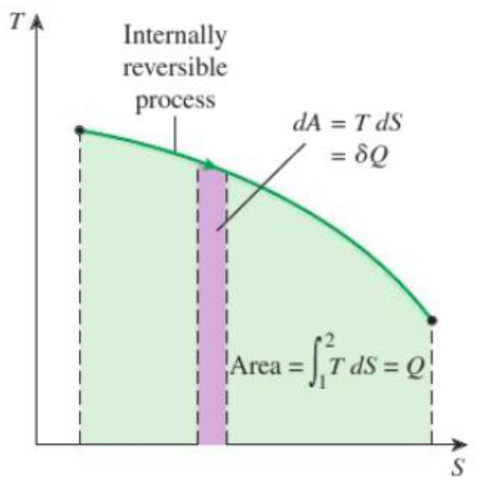
\includegraphics[scale=0.9]{./images/T-s-diagram.png}
\end{center}

\begin{itemize}
\item Differential form:
\[dS = \left(\frac{\delta Q}{T} \right)_{int rev} \quad \left(\unit{kJ.K^{-1}}\right)\]

\item Integrating:
\[Q_{int rev} = \int_1^2 T \, dS \left(\unit{kJ} \right)\]
\[q_{int rev} = \int_1^2 T \, ds \left(\unit{kJ} \right)\]

Where:
\begin{itemize}
\item \(Q_{int rev}\) is the heat transferred in an internally reversible process
\item \(T\) is the temperature in Kelvin
\item \(dS\) is the infinitesimal change in entropy
\item \(q_{int rev}\) is the specific heat transferred in an internally reversible process
\item \(ds\) is the infinitesimal change in specific entropy
\end{itemize}
\item \textbf{Area} under the \textbf{process curve} in the \textbf{T-s} diagram represents the \textbf{heat transfer} in an \textbf{internally reversible process}.
\item Internally reversible isothermal process:
\begin{center}
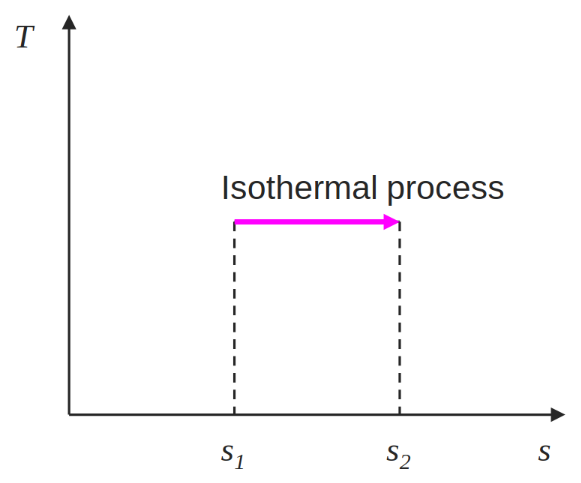
\includegraphics[scale=0.65]{./images/isothermal-process.png}
\end{center}

\[Q_{int rev} = T_0 \Delta S\]
\[q_{int rev} = T_0 \Delta s\]

Where:
\begin{itemize}
\item \(Q_{int rev}\) is the heat transferred in an internally reversible process
\item \(T\) is the temperature in Kelvin
\item \(\Delta S\) is the change in entropy
\item \(q_{int rev}\) is the specific heat transferred in an internally reversible process
\item \(\Delta s\) is the change in specific entropy
\end{itemize}

\item Isentropic process is a constant entropy process:
\begin{center}
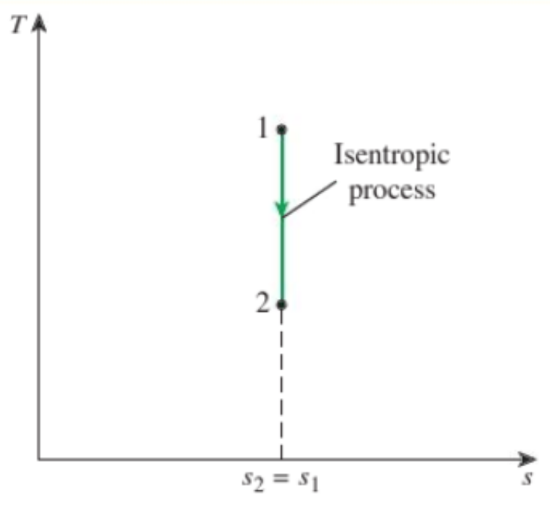
\includegraphics[scale=0.65]{./images/isentropic-process.png}
\end{center}
\end{itemize}

\subsubsection{\(h-s\) diagram (Mollier diagram)}
\label{sec:orgd70a361}
\begin{center}
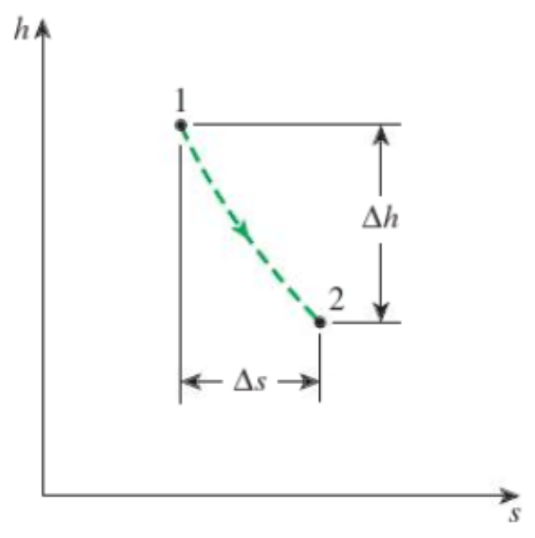
\includegraphics[scale=1]{./images/h-s-diagram.png}
\end{center}

\begin{itemize}
\item Useful in analysis of steady flow devices
\item Enthalpy \(h\) is the primary property in First Law analysis.
\item Entropy \(s\) is the property that accounts for irreversibilities in adiabatic processes.
\end{itemize}

\subsubsection{\(P-h\) diagram for water}
\label{sec:orge59bc47}
\begin{center}
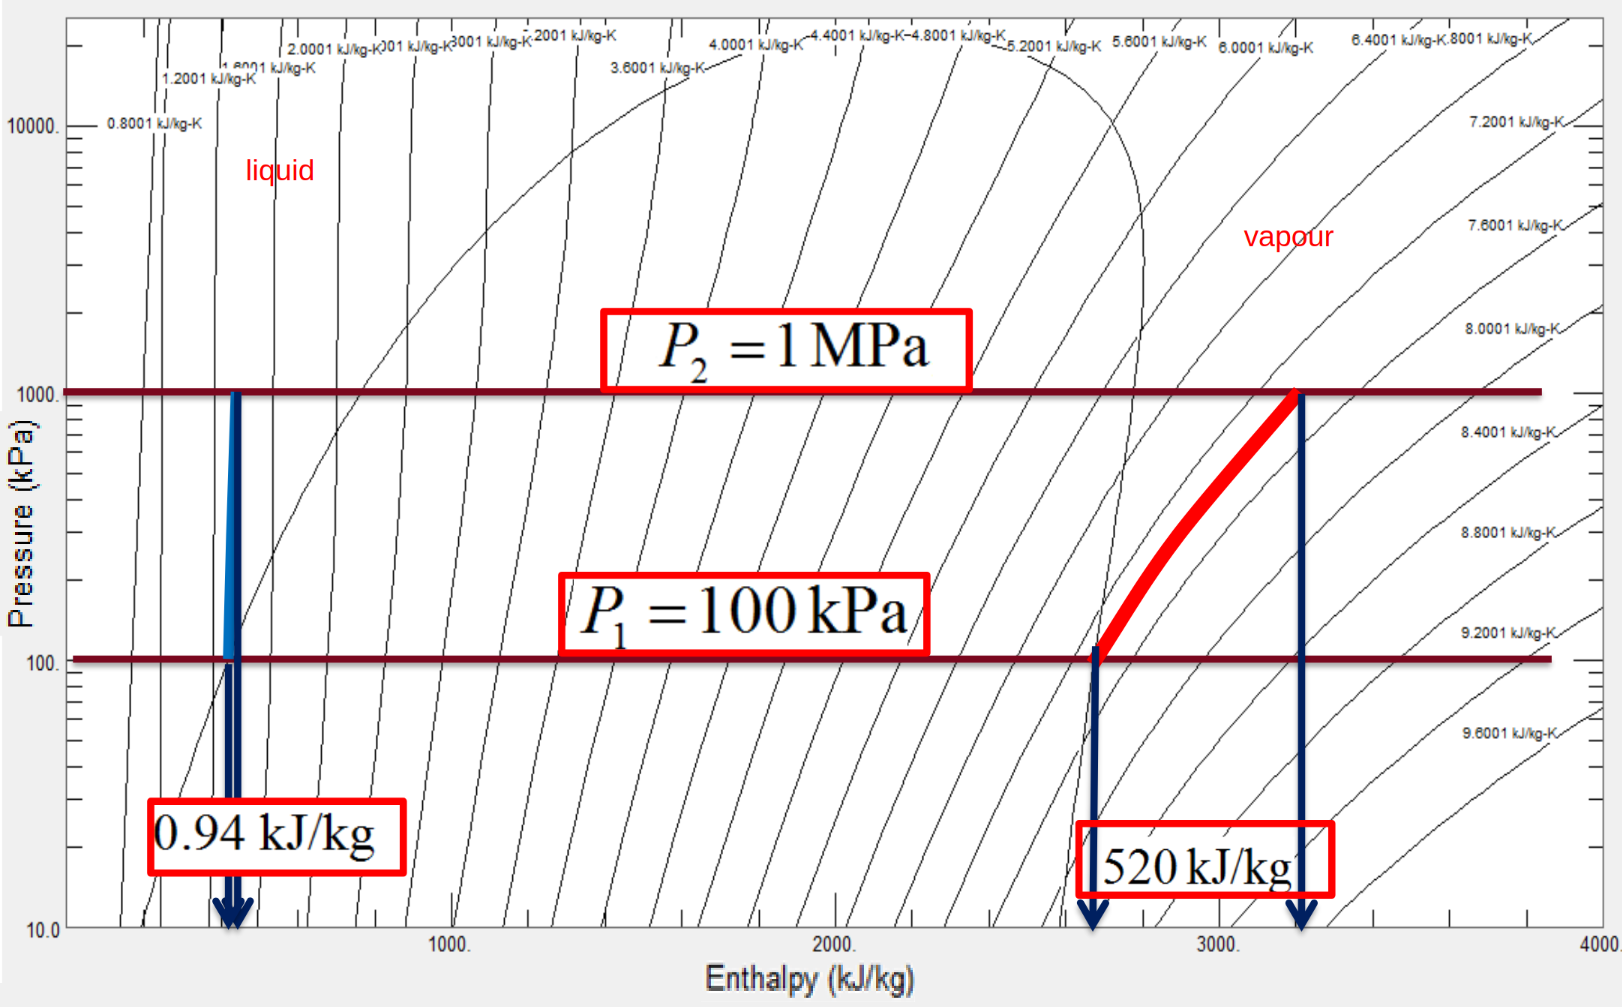
\includegraphics[width=.9\linewidth]{./images/P-h-diagram-for-water.png}
\end{center}

 \newpage

\section{Human comfort and air-conditioning}
\label{sec:org9a9d68f}
\begin{itemize}
\item Humans prefer comfortable environments that are neither too hot nor too cold, and neither too humid nor too dry.
\item The weather cannot be changed, but the climate in a confined space can be controlled.
\item Modern air-conditioning systems can do more than simply cooling or heating the air.
\begin{itemize}
\item Other functions include humification, dehumidification, cleaning and deodorisation, i.e. these systems condition the air.
\end{itemize}
\item A human body is like a heat engine:
\begin{itemize}
\item Rate of heat generation depends on the level of activity.
\item Waste heat is dissipated to the surroundings.
\item A body feels comfortable when it can dissipate its waste heat freely, and not more.
\item A body at rest dissipates about \(\qty{100}{W}\) when at rest.
\end{itemize}
\item Comfort of the human body depends primarily on three factors:
\begin{enumerate}
\item Dry-bulb temperature
\item Relative humidity
\item Air motion
\end{enumerate}
\item Relative humidity affects the amount of head a body can dissipate through sweat evaporation. \(40\% < \phi < 60\%\) is usually preferred
\item Air motion removes the build up of warm moist air around the body and replaces it with fresh air.
\item Air motion should be strong enough for such removal but gentle enough to be unnoticed.
\item If air motion is too strong, a chilling effect is produced (wind-chill factor).
\end{itemize}
\end{document}
